% *** Authors should verify (and, if needed, correct) their LaTeX system  ***
% *** with the testflow diagnostic prior to trusting their LaTeX platform ***
% *** with production work. IEEE's font choices can trigger bugs that do  ***
% *** not appear when using other class files.                            ***
% The testflow support page is at:
% http://www.michaelshell.org/tex/testflow/


%%*************************************************************************
%% Legal Notice:
%% This code is offered as-is without any warranty either expressed or
%% implied; without even the implied warranty of MERCHANTABILITY or
%% FITNESS FOR A PARTICULAR PURPOSE!
%% User assumes all risk.
%% In no event shall IEEE or any contributor to this code be liable for
%% any damages or losses, including, but not limited to, incidental,
%% consequential, or any other damages, resulting from the use or misuse
%% of any information contained here.
%%
%% All comments are the opinions of their respective authors and are not
%% necessarily endorsed by the IEEE.
%%
%% This work is distributed under the LaTeX Project Public License (LPPL)
%% ( http://www.latex-project.org/ ) version 1.3, and may be freely used,
%% distributed and modified. A copy of the LPPL, version 1.3, is included
%% in the base LaTeX documentation of all distributions of LaTeX released
%% 2003/12/01 or later.
%% Retain all contribution notices and credits.
%% ** Modified files should be clearly indicated as such, including  **
%% ** renaming them and changing author support contact information. **
%%
%% File list of work: IEEEtran.cls, New_IEEEtran_how-to.pdf, bare_jrnl_new_sample4.tex,
%%*************************************************************************
\PassOptionsToPackage{unicode}{hyperref}
\PassOptionsToPackage{hyphens}{url}
\PassOptionsToPackage{dvipsnames,svgnames,x11names}{xcolor}
% Note that the a4paper option is mainly intended so that authors in
% countries using A4 can easily print to A4 and see how their papers will
% look in print - the typesetting of the document will not typically be
% affected with changes in paper size (but the bottom and side margins will).
% Use the testflow package mentioned above to verify correct handling of
% both paper sizes by the user's LaTeX system.
%
% Also note that the "draftcls" or "draftclsnofoot", not "draft", option
% should be used if it is desired that the figures are to be displayed in
% draft mode.
%
\documentclass[
  journal,
]{IEEEtran}%
% If IEEEtran.cls has not been installed into the LaTeX system files,
% manually specify the path to it like:
% \documentclass[journal]{../sty/IEEEtran}
\usepackage[cmex10]{amsmath}
\usepackage{amssymb}
\usepackage{iftex}
\ifPDFTeX
  \usepackage[T1]{fontenc}
  \usepackage[utf8]{inputenc}
  \usepackage{textcomp} % provide euro and other symbols
\else % if luatex or xetex
  \usepackage{unicode-math} % this also loads fontspec
  \defaultfontfeatures{Scale=MatchLowercase}
  \defaultfontfeatures[\rmfamily]{Ligatures=TeX,Scale=1}
\fi
%\usepackage{lmodern}
\ifPDFTeX\else
\fi
% Use upquote if available, for straight quotes in verbatim environments
\IfFileExists{upquote.sty}{\usepackage{upquote}}{}
\IfFileExists{microtype.sty}{% use microtype if available
  \usepackage[]{microtype}
  \UseMicrotypeSet[protrusion]{basicmath} % disable protrusion for tt fonts
}{}
\makeatletter
\parindent    1.0em
\ifCLASSOPTIONcompsoc
  \parindent    1.5em
\fi
\makeatother
\usepackage{xcolor}
\setlength{\emergencystretch}{3em} % prevent overfull lines

\setcounter{secnumdepth}{5}
% Make \paragraph and \subparagraph free-standing
\ifx\paragraph\undefined\else
  \let\oldparagraph\paragraph
  \renewcommand{\paragraph}[1]{\oldparagraph{#1}\mbox{}}
\fi
\ifx\subparagraph\undefined\else
  \let\oldsubparagraph\subparagraph
  \renewcommand{\subparagraph}[1]{\oldsubparagraph{#1}\mbox{}}
\fi

\usepackage{longtable,booktabs,array}
\usepackage{calc} % for calculating minipage widths
% Correct order of tables after \paragraph or \subparagraph
\usepackage{etoolbox}
\makeatletter
\patchcmd\longtable{\par}{\if@noskipsec\mbox{}\fi\par}{}{}
\makeatother
% Allow footnotes in longtable head/foot
\IfFileExists{footnotehyper.sty}{\usepackage{footnotehyper}}{\usepackage{footnote}}
\makesavenoteenv{longtable}
\usepackage{graphicx}
\makeatletter
\newsavebox\pandoc@box
\newcommand*\pandocbounded[1]{% scales image to fit in text height/width
  \sbox\pandoc@box{#1}%
  \Gscale@div\@tempa{\textheight}{\dimexpr\ht\pandoc@box+\dp\pandoc@box\relax}%
  \Gscale@div\@tempb{\linewidth}{\wd\pandoc@box}%
  \ifdim\@tempb\p@<\@tempa\p@\let\@tempa\@tempb\fi% select the smaller of both
  \ifdim\@tempa\p@<\p@\scalebox{\@tempa}{\usebox\pandoc@box}%
  \else\usebox{\pandoc@box}%
  \fi%
}
% Set default figure placement to htbp
\def\fps@figure{htbp}
\makeatother


% definitions for citeproc citations
\NewDocumentCommand\citeproctext{}{}
\NewDocumentCommand\citeproc{mm}{%
  \begingroup\def\citeproctext{#2}\cite{#1}\endgroup}
\makeatletter
 % allow citations to break across lines
 \let\@cite@ofmt\@firstofone
 % avoid brackets around text for \cite:
 \def\@biblabel#1{}
 \def\@cite#1#2{{#1\if@tempswa , #2\fi}}
\makeatother
\newlength{\cslhangindent}
\setlength{\cslhangindent}{1.5em}
\newlength{\csllabelwidth}
\setlength{\csllabelwidth}{3em}
\newenvironment{CSLReferences}[2] % #1 hanging-indent, #2 entry-spacing
 {\begin{list}{}{%
  \setlength{\itemindent}{0pt}
  \setlength{\leftmargin}{0pt}
  \setlength{\parsep}{0pt}
  % turn on hanging indent if param 1 is 1
  \ifodd #1
   \setlength{\leftmargin}{\cslhangindent}
   \setlength{\itemindent}{-1\cslhangindent}
  \fi
  % set entry spacing
  \setlength{\itemsep}{#2\baselineskip}}}
 {\end{list}}
\usepackage{calc}
\newcommand{\CSLBlock}[1]{\hfill\break\parbox[t]{\linewidth}{\strut\ignorespaces#1\strut}}
\newcommand{\CSLLeftMargin}[1]{\parbox[t]{\csllabelwidth}{\strut#1\strut}}
\newcommand{\CSLRightInline}[1]{\parbox[t]{\linewidth - \csllabelwidth}{\strut#1\strut}}
\newcommand{\CSLIndent}[1]{\hspace{\cslhangindent}#1}



\setlength{\emergencystretch}{3em} % prevent overfull lines

\providecommand{\tightlist}{%
  \setlength{\itemsep}{0pt}\setlength{\parskip}{0pt}}



 


\usepackage{booktabs}
\usepackage{array}
\usepackage{physics}
\usepackage[version=3]{mhchem}
\usepackage{orcidlink}
\usepackage{float}
\floatplacement{table}{htb}
\makeatletter
\@ifpackageloaded{caption}{}{\usepackage{caption}}
\AtBeginDocument{%
\ifdefined\contentsname
  \renewcommand*\contentsname{Table of contents}
\else
  \newcommand\contentsname{Table of contents}
\fi
\ifdefined\listfigurename
  \renewcommand*\listfigurename{List of Figures}
\else
  \newcommand\listfigurename{List of Figures}
\fi
\ifdefined\listtablename
  \renewcommand*\listtablename{List of Tables}
\else
  \newcommand\listtablename{List of Tables}
\fi
\ifdefined\figurename
  \renewcommand*\figurename{Fig.}
\else
  \newcommand\figurename{Fig.}
\fi
\ifdefined\tablename
  \renewcommand*\tablename{Table}
\else
  \newcommand\tablename{Table}
\fi
}
\@ifpackageloaded{float}{}{\usepackage{float}}
\floatstyle{ruled}
\@ifundefined{c@chapter}{\newfloat{codelisting}{h}{lop}}{\newfloat{codelisting}{h}{lop}[chapter]}
\floatname{codelisting}{Listing}
\newcommand*\listoflistings{\listof{codelisting}{List of Listings}}
\makeatother
\makeatletter
\makeatother
\makeatletter
\@ifpackageloaded{caption}{}{\usepackage{caption}}
\@ifpackageloaded{subcaption}{}{\usepackage{subcaption}}
\makeatother
\usepackage[skip=2pt,font=footnotesize]{caption}
%\captionsetup{format=myformat}
\makeatletter
%\setlength{\cslhangindent}{0pt plus .5pt}
\providecommand{\bibfont}{\footnotesize}
\let\CSLReferences@rig=\CSLReferences
\renewcommand{\CSLReferences}[2]{
\bibfont\settowidth\csllabelwidth{[999]}
\CSLReferences@rig{#1}{#2}
\vskip 0.3\baselineskip plus 0.1\baselineskip minus 0.1\baselineskip%
}
\makeatother
\ifLuaTeX
  \usepackage{selnolig}  % disable illegal ligatures
\fi
\IfFileExists{bookmark.sty}{\usepackage{bookmark}}{\usepackage{hyperref}}
\IfFileExists{xurl.sty}{\usepackage{xurl}}{} % add URL line breaks if available
\urlstyle{same} % disable monospaced font for URLs
\hypersetup{
  pdftitle={Prioritising Technical Debt Without Source Code: A Multi-Criteria Framework on IT Service Management Data},
  pdfauthor={Zahid Ullah; Tobias Zeier},
  pdfkeywords={Configuration management database, financial services, IT
governance, IT service management, multi-criteria
decision-making, operational risk, technical debt, TOPSIS},
  colorlinks=true,
  linkcolor={blue},
  filecolor={Maroon},
  citecolor={Blue},
  urlcolor={Blue},
  pdfcreator={LaTeX via pandoc}}

% *** Do not adjust lengths that control margins, column widths, etc. ***
% *** Do not use packages that alter fonts (such as pslatex).         ***
% There should be no need to do such things with IEEEtran.cls V1.6 and later.
% (Unless specifically asked to do so by the journal or conference you plan
% to submit to, of course. )


% correct bad hyphenation here
\hyphenation{op-tical net-works semi-conduc-tor}

%
% paper title
% can use linebreaks \\ within to get better formatting as desired
% Do not put math or special symbols in the title.
% paper title
% can use linebreaks \\ within to get better formatting as desired
% Do not put math or special symbols in the title.
\title{Prioritising Technical Debt Without Source Code: A Multi-Criteria
Framework on IT Service Management Data}

\author{
Zahid Ullah
and~Tobias Zeier%
\thanks{Manuscript received XX Month 2026; revised XX Month 2026;
accepted XX Month 2026. (Corresponding author: Zahid Ullah.)Zahid Ullah
and Tobias Zeier are with the School of Computer Science and Electronic
Engineering, University of Essex, Colchester CO4 3SQ, U.K. (e-mail:
z.ullah@essex.ac.uk; tobi.zeier@gmail.com).This article extends the MSc
thesis of T. Zeier, completed under the supervision of Z. Ullah at the
University of Essex in 2026.}
\thanks{T. Zeier is also with the trading IT division of the case
organisation, a Swiss financial institution that is not named in this
article. Digital Object Identifier: to be assigned.}
}
\begin{document}

% The paper headers
\markboth{IEEE Transactions / IEEE Access, Vol. XX, No.~X, Month
2026}{Z. Ullah and T. Zeier: Prioritising Technical Debt Without Source
Code}

% use for special paper notices

% make the title area
\maketitle

% As a general rule, do not put math, special symbols or citations
% in the abstract or keywords.
\begin{abstract}
Technical debt (TD) is usually measured from source code, yet in
vendor-dominated financial IT the code is rarely accessible, and the
tools that depend on it leave infrastructure lifecycle, platform and
vulnerability debt largely unobserved. In mission-critical trading
systems this blind spot delays recovery, accumulates infrastructure risk
and weakens governance. This paper presents a service-level framework
that prioritises TD from operational records that organisations already
hold. Five indicators were derived from the literature and
operationalised from live IT service management (ITSM) and configuration
management database (CMDB) records: incident frequency, mean time to
recover, change failure rate, patch recency and unsupported component
months per component. The Technique for Order of Preference by
Similarity to Ideal Solution (TOPSIS) aggregates them into a ranked
remediation priority. The framework was applied to two years of
production data (2024 to 2025) from a systemically important Swiss
financial institution and evaluated analytically on six fronts: weight
sensitivity, convergent validity against simple additive weighting and
VIKOR, discriminant value against an incident-only baseline, rank
reversal under leave-one-out removal, indicator independence, and
practical readability of the ranked profiles. Rankings were stable under
weight variation (Kendall's tau of 0.867 in 2025), reproduced by
alternative methods and distinct from a single-criterion ordering. An
absolute-mode TOPSIS variant eliminated rank reversal by construction,
and a 20,000-sample Monte Carlo exploration of the weight space showed
that the lowest priority is weight-invariant while the top rank
concentrates on one service in 65\% of weightings. The framework offers
regulated institutions a transparent and reproducible instrument for ICT
risk decisions where source code cannot be reached.
\end{abstract}
% Note that keywords are not normally used for peerreview papers.
\begin{IEEEkeywords}
Configuration management database, financial services, IT governance, IT
service management, multi-criteria decision-making, operational
risk, technical debt, TOPSIS
\end{IEEEkeywords}

% For peer review papers, you can put extra information on the cover
% page as needed:
% \ifCLASSOPTIONpeerreview
% \begin{center} \bfseries EDICS Category: 3-BBND \end{center}
% \fi
%
% For peerreview papers, this IEEEtran command inserts a page break and
% creates the second title. It will be ignored for other modes.
% \IEEEpeerreviewmaketitle


\section{Introduction}\label{sec-intro}

\IEEEPARstart{T}{echnical} debt (TD) describes the implied future cost
of accepting short-term technical compromises over more robust solutions
\citeproc{ref-cunninghamWyCashPortfolioManagement1992}{{[}1{]}}. The
concept has expanded from source code quality to the architectural,
design, test, documentation and infrastructure dimensions of complex IT
systems \citeproc{ref-kruchtenTechnicalDebtMetaphor2012}{{[}2{]}}. Its
operational and financial consequences are measurable and compound
within a few years \citeproc{ref-bankerTechnicalDebtFirm2020}{{[}3{]}}.
In financial trading environments they are intensified by continuous
availability requirements, vendor-dominated architectures and regulatory
oversight \citeproc{ref-finmaCircular202312024}{{[}4{]}}. The absence of
a quantitative prioritisation mechanism is therefore particularly costly
in this setting \citeproc{ref-hakiDigitalNudgingTechnical2023}{{[}5{]}},
\citeproc{ref-ramasubbuControllingTechnicalDebt2021}{{[}6{]}}.

The literature does not yet offer a standardised, quantitative framework
for measuring and prioritising TD at the service level in
vendor-dominated enterprise IT. In a review of 44 primary studies,
Lenarduzzi et al.
\citeproc{ref-lenarduzziSystematicLiteratureReview2021}{{[}7{]}} found
that quantitative multi-criteria approaches are uncommon and that
empirical validation on industrial datasets is rare. Much of this gap
follows from where existing tools look. The dominant tools
operationalise debt as the remediation effort implied by source code
rule violations
\citeproc{ref-biazottoTechnicalDebtManagement2024}{{[}8{]}}. This makes
them inapplicable where source code is unavailable, as is typical for
the outsourced components and on-premises vendor software that form the
core of trading IT. Even where code can be accessed, tools run against
the same codebase return substantially divergent estimates
\citeproc{ref-amanatidisEvaluatingAgreementTechnical2020}{{[}9{]}}, and
they leave infrastructure lifecycle debt, platform obsolescence and
vulnerability debt largely unaddressed.

Operational data offers a route around this constraint. The four
delivery performance measures of the DevOps Research and Assessment
(DORA) programme are validated predictors of software delivery
performance \citeproc{ref-forsgrenAccelerate2018}{{[}10{]}}. The further
step from degraded operational indicators to elevated TD severity has
not been established empirically, so this study treats it as a testable
proposition rather than a premise. None of the work reviewed applies a
multi-criteria decision-making (MCDM) method to live service management
data in order to produce a ranked TD prioritisation instrument for
financial trading IT.

This paper closes that gap. It presents a service-level framework that
ranks IT services by TD priority using the Technique for Order of
Preference by Similarity to Ideal Solution (TOPSIS)
\citeproc{ref-hwangMultipleAttributeDecision1981}{{[}11{]}} on five
indicators drawn from live IT service management (ITSM) and
configuration management database (CMDB) records. The framework was
built and evaluated within the trading IT division of a systemically
important Swiss financial institution, following a design science
approach \citeproc{ref-hevnerDesignScienceInformation2004}{{[}12{]}}.
Three research questions guide the work.

\begin{itemize}
\tightlist
\item
  RQ1: How can TD in mission-critical trading systems be prioritised
  quantitatively at the service level using operational data?
\item
  RQ2: To what extent do operational service management metrics serve as
  valid proxies for TD severity in vendor-dominated enterprise IT?
\item
  RQ3: How stable are the resulting service rankings when criterion
  weights are perturbed?
\end{itemize}

The contributions are as follows. First, the paper proposes an
operationally defined indicator set with an explicit mapping to TD
dimensions, which can be extracted from ITSM and CMDB systems without
source code access. Second, it reports, to the best of our knowledge,
the first application of TOPSIS to live service management records for
TD prioritisation in financial trading IT. Third, it provides a
six-strand analytical evaluation covering weight sensitivity and
weight-space robustness, convergent and discriminant validity, rank
reversal, indicator independence and practical validity, and it shows
how an absolute-mode TOPSIS variant removes rank reversal in this
setting. Fourth, it documents a methodological finding of wider
relevance: vector-normalised TOPSIS can reward a service simply for
being the worst in the sample, whereas VIKOR and the absolute-mode
variant do not, and this difference can reorder the top of a ranking.

A note on terminology is in order. The framework measures debt
indirectly through operational proxies and expresses the result as a
relative priority. It produces a quantitative, reproducible ordering of
services by debt priority, not an absolute quantity of debt.

The remainder of the paper is organised as follows.
Section~\ref{sec-related} reviews the literature and states the research
gap. Section~\ref{sec-method} describes the research design, the
indicators, the TOPSIS formulation and the evaluation approach.
Section~\ref{sec-results} reports the data preparation and rankings.
Section~\ref{sec-evaluation} presents the evaluation.
Section~\ref{sec-discussion} answers the research questions and
discusses implications and threats to validity.
Section~\ref{sec-conclusion} concludes and identifies future work.

\section{Background and Related Work}\label{sec-related}

Four bodies of literature intersect at the problem addressed here: the
theory of TD, approaches to its measurement and prioritisation, its
governance in regulated financial IT and multi-criteria decision-making.
Sources were identified through Scopus, IEEE Xplore and Google Scholar
searches conducted between January and April 2026 and extended by
citation snowballing on three anchor publications
\citeproc{ref-kruchtenTechnicalDebtMetaphor2012}{{[}2{]}},
\citeproc{ref-lenarduzziSystematicLiteratureReview2021}{{[}7{]}},
\citeproc{ref-forsgrenAccelerate2018}{{[}10{]}}. The review is a
narrative synthesis, since the problem spans three disciplines with
differing evidence standards.

\subsection{The Expanding Perimeter of Technical
Debt}\label{the-expanding-perimeter-of-technical-debt}

Cunningham introduced the metaphor to explain a refactoring strategy to
non-technical stakeholders
\citeproc{ref-cunninghamWyCashPortfolioManagement1992}{{[}1{]}}.
McConnell distinguished principal, recurring interest and compounding
interest, and separated intentional from unintentional debt
\citeproc{ref-mcconnellManagingTechnicalDebt2008}{{[}13{]}}. Kruchten et
al.~formalised a taxonomy covering code, design, architectural, test,
build and documentation debt
\citeproc{ref-kruchtenTechnicalDebtMetaphor2012}{{[}2{]}}, which
underpins much subsequent empirical work. Developers in industrial
settings spend roughly 23\% of their time dealing with the consequences
of existing TD, with architectural debt exerting the strongest negative
influence on productivity
\citeproc{ref-beskerTechnicalDebtEmpirical2020}{{[}14{]}}. TD is also a
sociotechnical phenomenon in which communication failures drive
accumulation at least as much as technical decisions do
\citeproc{ref-ahmadTechnicalDebtNot2026}{{[}15{]}}, and in complex
systems it may never be fully removed
\citeproc{ref-vidoniInfiniteTechnicalDebt2022}{{[}16{]}}.

The perimeter of TD has widened well beyond source code. Kleinwaks et
al.~showed that requirements, architecture, integration and verification
artefacts all accumulate debt in systems engineering lifecycles
\citeproc{ref-kleinwaksTechnicalDebtSystems2023}{{[}17{]}}. Hanssen et
al.~identified regulatory change as a debt trigger, where architectural
decisions that were adequate before the Payment Services Directive 2
became sources of scalability debt once new requirements were imposed
\citeproc{ref-hanssenIdentifyingScalabilityDebt2019}{{[}18{]}}. Yang et
al.~proposed a taxonomy of debt for commercial off-the-shelf (COTS)
intensive systems that includes vendor platform obsolescence and
integration constraints
\citeproc{ref-yangTaxonomyTechnicalDebt2019}{{[}19{]}}. This broader
view matters for trading IT, where vendor platforms often form the core
of the operational stack and where platform, infrastructure and
vulnerability debt are invisible to static analysis.

\subsection{Measurement and
Prioritisation}\label{measurement-and-prioritisation}

Static analysis tools such as SonarQube, SQALE and CAST dominate TD
measurement, operationalising debt as estimated remediation effort
derived from rule violations. In a systematic mapping of 178 studies,
Biazotto et al.~found that most automated measurement artefacts remain
code-level, require substantial human intervention and rarely support
end-to-end TD management
\citeproc{ref-biazottoTechnicalDebtManagement2024}{{[}8{]}}. Industry
platforms such as SDK4ED integrate several code-level techniques but
offer little support for infrastructure and vendor-platform debt
\citeproc{ref-ampatzoglouSDK4EDPlatformTechnical2022}{{[}20{]}}, and the
business relevance of code quality, confirmed across 39 proprietary
codebases \citeproc{ref-tornhillCodeRedBusiness2022}{{[}21{]}}, does not
resolve the blind spots of a code-only view. Measurement consistency is
a further concern, since tools run against the same codebase return
substantially different estimates because each relies on its own ruleset
and thresholds
\citeproc{ref-amanatidisEvaluatingAgreementTechnical2020}{{[}9{]}}.
Infrastructure and process debt remain understudied relative to code and
architectural debt
\citeproc{ref-albuquerqueManagingTechnicalDebt2023}{{[}22{]}}.

Prioritisation shows the same lag. Lenarduzzi et al.~found that existing
approaches cluster around cost-based, value-based and risk-based
strategies, that most adopt a single primary criterion and that
quantitative methods are less common than heuristics
\citeproc{ref-lenarduzziSystematicLiteratureReview2021}{{[}7{]}}. The
operational stakes are concrete. De Toledo et al.~showed that targeted
repayment of architectural TD in a production microservices system
reduced incidents by 84\%
\citeproc{ref-detoledoReducingIncidentsMicroservices2021}{{[}23{]}}.
Practitioners weigh value and cost together rather than acting on a
single factor
\citeproc{ref-alfayezHowSonarQubeidentifiedTechnical2023}{{[}24{]}}, and
their decisions reflect technical severity, business impact and
available effort at once
\citeproc{ref-pinaTechnicalDebtPrioritization2022}{{[}25{]}}. Most IT
managers nonetheless lack a formal TD management process
\citeproc{ref-wieseITManagersPerspective2023}{{[}26{]}}. The Continuous
Debt Valuation Approach assigns a financial value to each debt item
\citeproc{ref-stochelBusinessdrivenTechnicalDebt2023}{{[}27{]}}, yet it
still relies on development-level data and ignores operational signals
such as incident rates or change failure rates. These are exactly the
signals that remain available where source code is inaccessible.

\subsection{Technical Debt in Regulated Financial
IT}\label{technical-debt-in-regulated-financial-it}

The most directly relevant precedent is the clinical research of Haki et
al.~at Credit Suisse, which defined a TD taxonomy spanning code quality,
infrastructure lifecycle, vulnerabilities and automation across more
than 3,000 applications
\citeproc{ref-hakiDigitalNudgingTechnical2023}{{[}5{]}}. Infrastructure
lifecycle debt was measured as cumulative months of unsupported
components, and vulnerability debt as weighted scanner-detected counts.
A major regulated institution thus treats both as operationally
significant categories measured through infrastructure records rather
than source code. Rolland and Lyytinen documented tensions at a large
Scandinavian bank between decentralised feature teams optimising local
throughput and the governance needed to manage debt at system level
\citeproc{ref-rollandExploringTensionsManagement2021}{{[}28{]}}. In both
cases organisational dynamics drive debt accumulation at least as much
as technical decisions do.

The enterprise systems literature adds firm-level evidence. A 10\%
increase in TD in COTS systems reduced gross return on assets by 16\% on
average, with the penalty more than doubling within six years
\citeproc{ref-bankerTechnicalDebtFirm2020}{{[}3{]}}. Across 1,824
outsourced remediation projects, client-vendor coordination only
improved outcomes when a long-term migration roadmap had been agreed
\citeproc{ref-ramasubbuControllingTechnicalDebt2021}{{[}6{]}}, and COTS
customisation creates self-reinforcing debt loops that code-level tools
cannot detect
\citeproc{ref-rinta-kahilaGettingTrappedTechnical2023}{{[}29{]}}.
Governance-level visibility of infrastructure debt is therefore required
before such loops become irreversible.

\subsubsection{Operational Indicators as Debt
Proxies}\label{operational-indicators-as-debt-proxies}

Forsgren et al.~showed, on survey data from over 2,000 organisations,
that mean time to recover (MTTR), change failure rate (CFR), deployment
frequency and lead time distinguish high-performing from low-performing
delivery organisations \citeproc{ref-forsgrenAccelerate2018}{{[}10{]}}.
Using these metrics as TD proxies requires the further claim that
degraded operational performance reflects accumulated debt rather than
staffing, immature release practices or organisational disruption. Nord
et al.~provide the most direct grounding for this step. They classify
delivery tempo degradation and deployment instability as observable TD
symptoms that manifest in production records, and they identify elevated
MTTR and CFR as signals that accumulated debt is impeding the system's
ability to absorb and recover from change
\citeproc{ref-nordExamplesTechnicalDebts2021}{{[}30{]}}. Paudel et
al.~found that TD density explained between 5\% and 41\% of lead time
variance across six fintech components, with team structure and
ownership as confounders
\citeproc{ref-paudelExploringRelationshipTechnical2025}{{[}31{]}}, which
argues for multi-criteria measurement rather than reliance on any single
proxy. Nielsen and Skaarup report that in a vendor-managed portfolio,
unsupported component versions surfaced only during infrastructure
migration rather than routine monitoring
\citeproc{ref-nielsenITPortfolioManagement2022}{{[}32{]}}.

Security-related debt is most visible in the patch management
literature. Enterprises delaying updates by one month faced 4.9 times
higher odds of compromise by advanced persistent threats, rising to 9.1
times at three months, and most campaigns exploited publicly known
vulnerabilities
\citeproc{ref-tizioSoftwareUpdatesStrategies2023}{{[}33{]}}. Patching
should therefore be treated as a risk-based business priority
\citeproc{ref-markkanenPatchManagementPlanning2023}{{[}34{]}} and as a
matter of contractual and service-level compliance
\citeproc{ref-nursePatchNotPatch2025}{{[}35{]}}, and keeping
dependencies current remains a persistent challenge in rapid-release
banking environments \citeproc{ref-kulaReleasingFastSlow2019}{{[}36{]}}.

Table~\ref{tbl-indicators-lit} summarises the mapping from operational
indicator to TD dimension used in this study. The dimension assignments
are our synthesis. Incident frequency is grounded in the incident and
reliability evidence of de Toledo et al.
\citeproc{ref-detoledoReducingIncidentsMicroservices2021}{{[}23{]}},
Ramasubbu and Kemerer
\citeproc{ref-ramasubbuControllingTechnicalDebt2021}{{[}6{]}},
\citeproc{ref-ramasubbuManagingTechnicalDebt2015}{{[}37{]}} and Nielsen
and Skaarup \citeproc{ref-nielsenITPortfolioManagement2022}{{[}32{]}}.
MTTR and CFR draw on Forsgren et al.
\citeproc{ref-forsgrenAccelerate2018}{{[}10{]}}, Nord et al.
\citeproc{ref-nordExamplesTechnicalDebts2021}{{[}30{]}} and Paudel et
al. \citeproc{ref-paudelExploringRelationshipTechnical2025}{{[}31{]}}.
Patch recency rests on Di Tizio et al.
\citeproc{ref-tizioSoftwareUpdatesStrategies2023}{{[}33{]}} and
Markkanen and Frantti
\citeproc{ref-markkanenPatchManagementPlanning2023}{{[}34{]}}, and
unsupported component months on Haki et al.
\citeproc{ref-hakiDigitalNudgingTechnical2023}{{[}5{]}}.

\begin{table}

\caption{\label{tbl-indicators-lit}Operational indicators mapped to TD
dimensions}

\centering{

\scriptsize
\setlength{\tabcolsep}{3pt}
\begin{tabular}{@{}>{\raggedright\arraybackslash}p{20mm}>{\raggedright\arraybackslash}p{20mm}>{\raggedright\arraybackslash}p{38mm}@{}}
\toprule
Indicator & TD dimension & Literature grounding \\
\midrule
Incident frequency & Architectural & de Toledo et al., Ramasubbu and Kemerer, Nielsen and Skaarup \\
Mean time to recover & Infrastructure and platform & Forsgren et al., Nord et al., Paudel et al. \\
Change failure rate & Process & Forsgren et al., Nord et al., Paudel et al. \\
Patch recency & Vulnerability & Di Tizio et al., Markkanen and Frantti \\
Unsupported component months & Infrastructure lifecycle & Haki et al. \\
\bottomrule
\end{tabular}

}

\end{table}%

\subsection{Multi-Criteria Decision-Making and
TOPSIS}\label{multi-criteria-decision-making-and-topsis}

Prioritising TD involves balancing remediation cost, operational risk,
security exposure and regulatory compliance at once, which is the class
of problem MCDM methods address. Simple additive weighting (SAW) scores
each alternative as a weighted sum across the criteria. It is
transparent but fully compensatory. TOPSIS, introduced by Hwang and Yoon
\citeproc{ref-hwangMultipleAttributeDecision1981}{{[}11{]}}, scores each
alternative by its distance to both an ideal best and an ideal worst
solution. Ciardiello and Genovese show that under some distance metrics
TOPSIS reproduces SAW closely
\citeproc{ref-ciardielloComparisonTOPSISSAW2023}{{[}38{]}}, so method
choice is treated here as a robustness question rather than one of
correctness. In a simulation comparing eight methods, Zanakis et
al.~found TOPSIS the most robust to rank reversal among the methods that
exhibit it
\citeproc{ref-zanakisMultiattributeDecisionMaking1998}{{[}39{]}}.

Rank reversal remains a documented limitation. Adding or removing an
alternative can reorder the others, because vector normalisation and the
ideal solutions both depend on the current set
\citeproc{ref-garcia-cascalesRankReversalTOPSIS2012}{{[}40{]}}. The same
authors propose an absolute-mode correction that anchors normalisation
and the ideal solutions to fixed bounds, and Yang proves that variants
with set-independent bounds and ideals are ranking stable by
construction \citeproc{ref-yangIngeniousSolutionRank2020}{{[}41{]}}.
VIKOR identifies compromise solutions and fits less well where a
complete ranked list is required
\citeproc{ref-shekhovtsovComparativeCaseStudy2020}{{[}42{]}}.
Shekhovtsov and Sałabun also show that method choice matters less than
weight specification when weights are uncertain
\citeproc{ref-shekhovtsovComparativeCaseStudy2020}{{[}42{]}}, which
underlines the importance of transparent weight determination and of the
robustness analysis that Greco et al.~recommend for composite indicators
\citeproc{ref-grecoMethodologicalFrameworkComposite2019}{{[}43{]}}.

Albarak et al.~provide the most directly analogous precedent, combining
TOPSIS with portfolio theory to prioritise database normalisation debt
and showing that it surfaces high-priority items likely to be deferred
under effort-only approaches
\citeproc{ref-albarakManagingTechnicalDebt2022}{{[}44{]}}. TOPSIS has
also been applied in other regulated, risk-intensive settings
\citeproc{ref-zytoonDecisionSupportModel2020}{{[}45{]}},
\citeproc{ref-khanIntegratedMethodologyRanking2022}{{[}46{]}}. None of
these operates on live service management data in a financial
enterprise.

\subsection{Research Gap}\label{research-gap}

Related work does not offer a framework integrating service-level
operational indicators, multi-criteria prioritisation and the
constraints of regulated financial trading IT into a single auditable
ranking instrument. Code-centric tools are structurally inapplicable to
vendor-hosted platforms, and single-criterion models conflict with both
practitioner behaviour and the multidimensional nature of operational
risk. Existing TOPSIS applications to TD rely on controlled datasets.
The framework developed here applies TOPSIS to five operational
indicators from live ITSM and CMDB records and evaluates the result
following the logic of Greco et al.
\citeproc{ref-grecoMethodologicalFrameworkComposite2019}{{[}43{]}} and
Albarak et al.
\citeproc{ref-albarakManagingTechnicalDebt2022}{{[}44{]}}.

\section{Research Method}\label{sec-method}

\subsection{Research Design and Case
Setting}\label{research-design-and-case-setting}

The study adopts a pragmatist stance, under which the value of a
knowledge claim rests on whether the resulting artefact works in the
context it was designed for
\citeproc{ref-kellyThreePrinciplesPragmatism2020}{{[}47{]}}. It follows
the design science research (DSR) guidelines of Hevner et al.
\citeproc{ref-hevnerDesignScienceInformation2004}{{[}12{]}} and the
six-step process of Peffers et al.
\citeproc{ref-peffersDesignScienceResearch2007}{{[}48{]}}: problem
identification, definition of objectives, design and development,
demonstration, evaluation and communication. The artefact is a
TOPSIS-based prioritisation framework operating on live ITSM and CMDB
data. The sequence was not strictly linear, since indicator selection
and evaluation criteria were refined when constraints in the available
data emerged.

The empirical setting is a single-organisation embedded case study
within the trading IT division of a systemically important Swiss
financial institution. The unit of analysis is the individual IT
service, defined as a distinct configuration item in the organisation's
ITSM instance. The design is cross-sectional within each observation
year, with two years analysed (January 2024 to December 2025) to allow a
temporal comparison. Three factors make this design appropriate. The
regulatory, operational and vendor-platform characteristics of Swiss
financial IT resist generalisation from studies conducted elsewhere.
Granular ITSM records are unavailable through surveys or experiments.
Evaluating the artefact against operational data from its target
environment satisfies the rigorous evaluation requirement of DSR.

Ethical and professional considerations shaped the design. The data
originate from a live institution that is not identified by name. All
service, team and vendor identifiers were replaced with alphanumeric
codes before analysis, and no employee data are present, since all
indicators are service-level aggregates. The second author is employed
in the trading IT division of the case organisation, which is how access
to the records was obtained. The data-sharing arrangement was authorised
by the Head of Trading IT, only the fields required for the five
indicators were exported, and no records were retained beyond the
analytical period. The dataset contains no personal data under the
revised Swiss Federal Act on Data Protection
\citeproc{ref-FederalActData2023}{{[}49{]}}, and data minimisation was
applied nonetheless. The institution is subject to FINMA Circular 2023/1
on operational risks and resilience
\citeproc{ref-finmaCircular202312024}{{[}4{]}}. The metrics used are
organisationally defined rather than prescribed by the regulator. The
governance scope was agreed at the outset: the framework supports a
portfolio-level view of service health and informs governance
conversations, and it was not shared with service teams during the
research period. The study followed the BCS Code of Conduct
\citeproc{ref-CodeConductBCS2022}{{[}50{]}}.

\subsection{Indicator Selection and Operational
Definitions}\label{sec-indicators}

The literature review identified candidate indicators mapping TD
dimensions to operational data (Table~\ref{tbl-indicators-lit}). A data
audit against available ITSM and CMDB fields refined this set.
Documentation completeness was excluded because no structured field
captures it consistently. Test coverage and architectural coupling were
excluded because both require build artefacts, source repositories or
compiled code, none of which is accessible for vendor-managed or
outsourced components
\citeproc{ref-amanatidisEvaluatingAgreementTechnical2020}{{[}9{]}}. Raw
vulnerability density was excluded in favour of patch recency on data
availability grounds. Table~\ref{tbl-indicators-def} lists the five
retained indicators.

\begin{table}

\caption{\label{tbl-indicators-def}Operational indicator definitions}

\centering{

\scriptsize
\setlength{\tabcolsep}{3pt}
\begin{tabular}{@{}>{\raggedright\arraybackslash}p{16mm}>{\raggedright\arraybackslash}p{30mm}>{\raggedright\arraybackslash}p{9mm}>{\raggedright\arraybackslash}p{14mm}>{\raggedright\arraybackslash}p{9mm}@{}}
\toprule
Indicator & Operational definition & Source & Unit & Dir. \\
\midrule
Incident frequency & Incidents per service per year & ITSM & Incidents per year & Cost \\
MTTR & Arithmetic mean incident resolution time & ITSM & Hours & Cost \\
CFR & Weighted incidents divided by number of changes & ITSM & Ratio & Cost \\
Patch recency & Share of components within a supported release window & CMDB & \% (0 to 100) & Benefit \\
Unsupported component months & Months of exposure to unsupported components divided by component count & CMDB & Months per component & Cost \\
\bottomrule
\end{tabular}

}

\end{table}%

Two caveats apply. Incident frequency and MTTR are computed from all
recorded incidents irrespective of severity. CFR is a derived proxy that
follows the formula the case organisation itself applies, in which
incidents are weighted by severity class and divided by the number of
changes in the period: \begin{equation}\label{eq:cfr}
\text{CFR} = \frac{100\,n_1 + 10\,n_2 + n_3 + 0.1\,n_4}{\text{number of changes}},
\end{equation} where \(n_k\) is the number of severity-\(k\) incidents
and severity 1 is the most critical class. Severity 1 incidents are
extremely rare in the case organisation, so the measure is driven in
practice by severity 2 and 3 incidents. It approximates the DORA change
failure rate without the deployment-outcome labelling a true CFR
requires, and because it shares its incident numerator with incident
frequency, the two criteria are not fully independent. The extent of
this dependence is quantified in Section~\ref{sec-independence} and its
effect on the ordering is bounded by the weight sensitivity analysis in
Section~\ref{sec-stability}.

The CMDB-derived indicators operationalise vulnerability and
infrastructure lifecycle debt following Haki et al.
\citeproc{ref-hakiDigitalNudgingTechnical2023}{{[}5{]}}. Unsupported
component months requires one normalisation before entering the decision
matrix. In raw form it grows with the number of components a service
comprises, so a large estate carrying a few unsupported components would
outscore a compact service whose whole stack is out of support
\citeproc{ref-ampatzoglouReusabilityIndexMeasure2018}{{[}51{]}}. It is
therefore converted to a size-relative intensity, as in
\eqref{eq:intensity}, a standard exposure normalisation step for
composite indicators whose sub-indicators differ in size dependence
\citeproc{ref-grecoMethodologicalFrameworkComposite2019}{{[}43{]}},
\citeproc{ref-nardoToolsCompositeIndicators2005}{{[}52{]}}:
\begin{equation}\label{eq:intensity}
u_i = \frac{(\text{unsupported component months})_i}{(\text{component count})_i}.
\end{equation} An intensity is preferred over a simple share of
unsupported components because it preserves both how many components are
affected and for how long. A fully supported service scores zero
regardless of size. This step is separate from, and applied before, the
vector normalisation inside TOPSIS.

\subsection{TOPSIS Formulation}\label{sec-topsis}

Given a decision matrix \(X = [x_{ij}]\) with \(m\) services and \(n\)
indicators, the standard procedure
\citeproc{ref-hwangMultipleAttributeDecision1981}{{[}11{]}},
\citeproc{ref-pandeyReviewTOPSISMethod2023}{{[}53{]}} proceeds in five
steps. Each value is first scaled relative to its column norm, which
removes differences in unit and range: \begin{equation}\label{eq:norm}
r_{ij} = \frac{x_{ij}}{\sqrt{\sum_{i=1}^{m} x_{ij}^2}}.
\end{equation} The weighted normalised matrix is formed with criterion
weights \(w_j\), where \(\sum_j w_j = 1\):
\begin{equation}\label{eq:weighted}
v_{ij} = w_j \, r_{ij}.
\end{equation} The positive and negative ideal solutions
\(A^{+} = \{v_1^{+}, \ldots, v_n^{+}\}\) and
\(A^{-} = \{v_1^{-}, \ldots, v_n^{-}\}\) collect, for each criterion,
the best and worst weighted normalised values observed across the
services, respecting criterion direction. Euclidean distances to each
ideal are then \begin{equation}\label{eq:dist}
S_i^{+} = \sqrt{\sum_{j=1}^{n}(v_{ij} - v_j^{+})^2}, \qquad
S_i^{-} = \sqrt{\sum_{j=1}^{n}(v_{ij} - v_j^{-})^2},
\end{equation} and the relative closeness coefficient is
\begin{equation}\label{eq:closeness}
C_i = \frac{S_i^{-}}{S_i^{+} + S_i^{-}}, \qquad C_i \in [0, 1].
\end{equation} A higher \(C_i\) indicates that a service is closer to
the ideal operational profile and therefore has lower TD priority.
Incident frequency, MTTR, CFR and unsupported component months are cost
criteria, and patch recency is a benefit criterion. Services are ranked
by \(C_i\) in ascending order, so rank 1 denotes the highest remediation
priority.

\subsection{Absolute-Mode Variant}\label{absolute-mode-variant}

The evaluation also uses an absolute-mode variant of TOPSIS that is
invariant to the set of services being ranked, following García-Cascales
and Lamata
\citeproc{ref-garcia-cascalesRankReversalTOPSIS2012}{{[}40{]}} and Yang
\citeproc{ref-yangIngeniousSolutionRank2020}{{[}41{]}}. Two elements of
the standard procedure are replaced. First, vector normalisation
\eqref{eq:norm} is replaced by normalisation against fixed bounds. Each
criterion \(j\) is assigned a range \([l_j, u_j]\) with a floor \(l_j\)
(zero in this study) and an upper bound \(u_j\) declared from
organisational thresholds rather than from the sample:
\begin{equation}\label{eq:absnorm}
r^{\text{abs}}_{ij} = \frac{x_{ij} - l_j}{u_j - l_j}.
\end{equation} Second, the ideal solutions are anchored to the extremes
of each criterion scale in the weighted normalised space rather than to
the observed best and worst values: \begin{equation}\label{eq:absideal}
v_j^{+} =
\begin{cases}
w_j, & j \text{ benefit} \\
0,   & j \text{ cost}
\end{cases}
\qquad
v_j^{-} =
\begin{cases}
0,   & j \text{ benefit} \\
w_j, & j \text{ cost.}
\end{cases}
\end{equation} Because the bounds and both ideal components are fixed,
they do not change when a service is added or removed, so the ranking is
invariant to portfolio composition. Distances and the closeness
coefficient are computed as in \eqref{eq:dist} and \eqref{eq:closeness}.
The variant is used for the leave-one-out rank-reversal test and as the
scorer for the weight-space analysis. The declared bounds are listed in
Table~\ref{tbl-bounds}. Each upper bound is an organisational threshold
beyond which the service would be treated as outside normal operating
conditions, and all observed values fall within them.

\begin{table}

\caption{\label{tbl-bounds}Fixed criterion bounds for absolute-mode
TOPSIS}

\centering{

\scriptsize
\setlength{\tabcolsep}{4pt}
\begin{tabular}{@{}lrr@{}}
\toprule
Criterion & $l_j$ & $u_j$ \\
\midrule
Incident frequency (per year) & 0 & 1000 \\
MTTR (hours) & 0 & 120 \\
CFR & 0 & 5 \\
Patch recency (\%) & 0 & 100 \\
Unsupported months per component & 0 & 30 \\
\bottomrule
\end{tabular}

}

\end{table}%

\subsection{Weight Configurations}\label{weight-configurations}

Two weight configurations are used (Table~\ref{tbl-weights}). A baseline
equal-weight configuration (\(w_j = 0.20\)) serves as the reference
against which the second configuration is compared. Equal weighting is
the standard default in composite indicator construction in the absence
of empirically justified differential weights
\citeproc{ref-grecoMethodologicalFrameworkComposite2019}{{[}43{]}}. A
differential configuration assigns higher weight to MTTR and patch
recency (\(w_j = 0.30\) each) and lower weight to the remaining three
indicators (\(w_j = 0.1\overline{3}\) each). This reflects a
practitioner judgement that recovery time and delayed patching carry
greater operational consequence in time-critical trading environments.
The configuration is not derived from literature and is treated as an
explicit assumption whose influence is assessed in
Section~\ref{sec-evaluation}.

\begin{table}

\caption{\label{tbl-weights}Weight configurations}

\centering{

\scriptsize
\setlength{\tabcolsep}{4pt}
\begin{tabular}{@{}lrrrrr@{}}
\toprule
Configuration & Inc. freq. & MTTR & CFR & Patch rec. & Unsup. months \\
\midrule
Equal (baseline) & 0.20 & 0.20 & 0.20 & 0.20 & 0.20 \\
Differential & $0.1\overline{3}$ & 0.30 & $0.1\overline{3}$ & 0.30 & $0.1\overline{3}$ \\
\bottomrule
\end{tabular}

}

\end{table}%

\subsection{Evaluation Approach}\label{sec-evalapproach}

No external ground-truth measure exists for the non-code debt this
framework targets. Code-level tools disagree on the same codebase
\citeproc{ref-amanatidisEvaluatingAgreementTechnical2020}{{[}9{]}} and
leave infrastructure, platform and vulnerability debt weakly observed
\citeproc{ref-biazottoTechnicalDebtManagement2024}{{[}8{]}},
\citeproc{ref-albuquerqueManagingTechnicalDebt2023}{{[}22{]}}, and the
agreed governance scope precluded interviewing service teams. The
framework is therefore evaluated analytically in the sense of Hevner et
al. \citeproc{ref-hevnerDesignScienceInformation2004}{{[}12{]}},
establishing robustness, method-independence and discriminant value
rather than criterion validity.

Six strands are applied. Ranking stability tests whether the order
survives weight variation and holds across observation years, extended
by a Monte Carlo exploration of the full weight space
\citeproc{ref-grecoMethodologicalFrameworkComposite2019}{{[}43{]}}.
Convergent validity re-ranks the same services with SAW and VIKOR and
measures agreement with the TOPSIS order
\citeproc{ref-ciardielloComparisonTOPSISSAW2023}{{[}38{]}},
\citeproc{ref-shekhovtsovComparativeCaseStudy2020}{{[}42{]}}.
Discriminant value compares the composite ordering against a
single-criterion ranking by incident frequency, following Albarak et al.
\citeproc{ref-albarakManagingTechnicalDebt2022}{{[}44{]}}. Structural
rigour removes services one at a time and checks whether the order of
the remainder holds, which addresses rank reversal
\citeproc{ref-garcia-cascalesRankReversalTOPSIS2012}{{[}40{]}}.
Indicator independence examines the correlation structure among the five
indicators to establish how many distinct signals the composite
aggregates. Practical validity reads the rankings against the service
profiles they describe. Agreement between rankings is measured
throughout with Kendall's \(\tau\), which is well established in MCDM
evaluation \citeproc{ref-shekhovtsovHowStronglyRank2021}{{[}54{]}}.

\section{Framework Application and Results}\label{sec-results}

\subsection{Data Preparation}\label{data-preparation}

The trading IT portfolio comprises 108 services. Fifty-three are small
vendor applications, such as vendor graphical user interfaces, and were
excluded because they require no significant ongoing activity from the
portfolio's IT teams. From the remaining services, six were selected for
demonstration on the basis of data completeness. Each holds a continuous
record across all five indicators for the full two-year window in both
systems, is registered as an active configuration item and has been in
operation for more than thirty-six months. Two consequences follow from
such a small demonstration set. The services selected tend to carry
higher operational activity, so absolute indicator values are not
representative of the full portfolio, and a six-service decision matrix
limits the discriminatory power of the rank-stability tests. The
contribution is therefore the working instrument and its evaluation
logic rather than a portfolio-wide ranking.

The indicators were extracted from the organisation's ITSM instance and
CMDB on 11 June 2026, with only production records included. Several
quality filters were applied to the raw incident data. Incidents sharing
a common root cause but recorded as separate tickets, a pattern typical
of alarm storms, were consolidated into a single incident. Incidents
with a resolution time below 0.1 hours were excluded, since resolutions
at that speed most likely reflect automatic closure after a false alarm.
A 98th percentile cap addressed the upper tail of the MTTR distribution,
excluding incidents whose resolution times more plausibly reflect
administrative inactivity than active resolution effort. Together the
three filters removed {[}N{]} of the {[}M{]} raw incident records across
the two years, {[}X{]}\% of the total, so they corrected the tails
without reshaping the distribution. All CMDB records were complete, so
no imputation was required. The cumulative unsupported-component-months
figure was divided by each service's registered component count
according to \eqref{eq:intensity}, with numerator and denominator drawn
from the same extract.

The data carry inherent quality limitations. Incident frequency, MTTR
and CFR depend on the accuracy and completeness of the incidents opened
and closed. Recording practices vary across teams: some contacts arrive
by phone, email or chat and become a formal ITSM record only at the
receiving team's discretion, while others are handled in a separate
issue tracker and never escalated. Services where informal handling is
common may therefore record lower incident counts and CFR values than
their true failure rate warrants. MTTR is exposed at closure, since a
team that leaves resolved incidents open will show a longer mean than
its actual recovery warrants. Patch recency is bounded by CMDB coverage
and scanner configuration, and the accuracy of the CMDB component count
is a dependency of the per-component intensity. Scores should
accordingly be read as ordinal priority signals rather than exact
measurements, and Section~\ref{sec-evaluation} tests whether the ranking
is robust to the input variation these limitations may introduce.

\subsection{Indicator Values}\label{indicator-values}

Table~\ref{tbl-raw-data} presents the extracted indicator values for
2025. The services differ markedly in profile. SVC-04 carries by far the
highest incident frequency but has a fully supported, fully patched
stack. SVC-06 combines the second-highest incident count with the worst
CFR, the worst patch recency and the heaviest per-component lifecycle
exposure. SVC-03 is well maintained on every indicator.

\begin{table}

\caption{\label{tbl-raw-data}Indicator values per service, 2025}

\centering{

\scriptsize
\setlength{\tabcolsep}{4pt}
\begin{tabular}{@{}lrrrrr@{}}
\toprule
Service & \shortstack[r]{Inc. freq.\\(per year)} & \shortstack[r]{MTTR\\(h)} & CFR & \shortstack[r]{Patch rec.\\(\%)} & \shortstack[r]{Unsup. months\\per comp.} \\
\midrule
SVC-01 & 64 & 45.35 & 0.83 & 53.10 & 5.67 \\
SVC-02 & 30 & 25.26 & 0.19 & 61.90 & 2.42 \\
SVC-03 & 21 & 13.31 & 0.38 & 100.00 & 0.00 \\
SVC-04 & 574 & 41.91 & 3.38 & 100.00 & 0.00 \\
SVC-05 & 171 & 23.72 & 1.52 & 100.00 & 0.00 \\
SVC-06 & 302 & 13.11 & 3.96 & 52.94 & 18.88 \\
\bottomrule
\end{tabular}

}

\end{table}%

\subsection{TOPSIS Rankings}\label{topsis-rankings}

The computation follows \eqref{eq:norm} to \eqref{eq:closeness} and was
executed in a Python implementation. Table~\ref{tbl-results2025}
presents the 2025 results under both weight configurations, sorted from
highest to lowest debt priority. Table~\ref{tbl-results2024} presents
the corresponding 2024 results, computed with the same configurations to
allow a temporal comparison.

\begin{table}

\caption{\label{tbl-results2025}TOPSIS results, 2025 (higher \(C_i\),
lower debt priority)}

\centering{

\scriptsize
\setlength{\tabcolsep}{5pt}
\begin{tabular}{@{}lrrrr@{}}
\toprule
Service & $C_i$ (equal) & Rank & $C_i$ (differential) & Rank \\
\midrule
SVC-06 & 0.3204 & 1 & 0.4415 & 1 \\
SVC-04 & 0.4778 & 2 & 0.4512 & 2 \\
SVC-01 & 0.6619 & 3 & 0.4976 & 3 \\
SVC-05 & 0.7790 & 4 & 0.7615 & 5 \\
SVC-02 & 0.8297 & 5 & 0.7175 & 4 \\
SVC-03 & 0.9774 & 6 & 0.9809 & 6 \\
\bottomrule
\end{tabular}

}

\end{table}%

\begin{table}

\caption{\label{tbl-results2024}TOPSIS results, 2024 (higher \(C_i\),
lower debt priority)}

\centering{

\scriptsize
\setlength{\tabcolsep}{5pt}
\begin{tabular}{@{}lrrrr@{}}
\toprule
Service & $C_i$ (equal) & Rank & $C_i$ (differential) & Rank \\
\midrule
SVC-04 & 0.4837 & 1 & 0.5038 & 1 \\
SVC-06 & 0.5163 & 2 & 0.6048 & 3 \\
SVC-02 & 0.6999 & 3 & 0.5102 & 2 \\
SVC-05 & 0.7058 & 4 & 0.7092 & 5 \\
SVC-01 & 0.7759 & 5 & 0.6231 & 4 \\
SVC-03 & 0.8492 & 6 & 0.8816 & 6 \\
\bottomrule
\end{tabular}

}

\end{table}%

The dominant lifecycle-debt signal sits with SVC-06 in both years. Its
per-component exposure is the highest in the portfolio, at 16.41 months
per component in 2024 and 18.88 in 2025, and by 2025 this combines with
the worst CFR and the worst patch recency to place it first for
remediation under both configurations. SVC-01's exposure also rose year
on year, from 0.24 to 5.67 months per component, but spread across a
large component base it remains a second-order signal. Together with the
portfolio's highest MTTR and second-worst patch recency it places SVC-01
third in 2025. This illustrates the effect of the per-component
normalisation directly. Under a cumulative measure, SVC-01's large
estate would have produced the biggest raw figure and drawn it to the
top of the ranking, whereas the size-adjusted intensity subordinates it
to SVC-06, a compact service about half out of support, and for far
longer.

\section{Evaluation}\label{sec-evaluation}

Before the ordering in Section~\ref{sec-results} is interpreted, it must
earn trust. This section tests it on the six fronts set out in
Section~\ref{sec-evalapproach}. With only six services, the \(p\)-values
for Kendall's \(\tau\) are obtained exactly across all \(6! = 720\)
orderings. The small sample limits the power of the test, but the
limitation reflects portfolio size rather than weak agreement, since
\(p\)-values fall as the sample grows when a real effect is present
\citeproc{ref-chenRolesChallengesMerits2023}{{[}55{]}}. The \(p\)-values
are therefore read as effect sizes rather than accept-or-reject
decisions.

\subsection{Ranking Stability}\label{sec-stability}

Table~\ref{tbl-kendall} reports Kendall's \(\tau\) for the standard
TOPSIS formulation. Weight sensitivity is high in both years
(\(\tau = 0.867\) in 2025, \(0.733\) in 2024). Reweighting MTTR and
patch recency leaves the priority order largely intact, moving only
adjacent mid-field services. Temporal stability is moderate
(\(\tau = 0.467\) equal, \(0.600\) differential), and the movement
follows real profile change. SVC-06 carries the portfolio's heaviest
per-component lifecycle exposure in both years. Ranked second in 2024,
it rises to the top priority in 2025 as its CFR and patch position
deteriorate. SVC-01 climbs from fifth in 2024 to third in 2025 as its
patch recency collapses and its per-component unsupported exposure
rises. Cross-year movement is reported as descriptive context rather
than as a quality criterion in its own right, since services evolve
between periods and a faithful ranking should follow that change. In
every run the lowest-priority position is identical, and the same three
services occupy the high-priority half in 2025 under both
configurations.

\begin{table}

\caption{\label{tbl-kendall}Kendall's \(\tau\) across ranking
comparisons, standard TOPSIS}

\centering{

\scriptsize
\setlength{\tabcolsep}{4pt}
\begin{tabular}{@{}>{\raggedright\arraybackslash}p{58mm}rr@{}}
\toprule
Comparison & $\tau$ & $p$ \\
\midrule
Weight sensitivity 2025 (equal vs differential) & 0.867 & 0.017 \\
Weight sensitivity 2024 (equal vs differential) & 0.733 & 0.056 \\
Temporal stability, equal weights (2025 vs 2024) & 0.467 & 0.272 \\
Temporal stability, differential weights (2025 vs 2024) & 0.600 & 0.136 \\
\bottomrule
\end{tabular}

}

\end{table}%

\subsection{Convergent Validity Across Methods}\label{sec-convergent}

To test whether the ordering depends on the choice of method, the six
services were re-ranked with SAW and VIKOR and compared against standard
and absolute-mode TOPSIS. SAW used min-max (Weitendorf) normalisation to
avoid the division by zero that classic cost normalisation would produce
on the dataset's zero values
\citeproc{ref-thienOvercomingLimitationsRAPS2024}{{[}56{]}}. VIKOR
followed the standard \(S\), \(R\) and \(Q\) procedure with \(v = 0.5\).

Table~\ref{tbl-convergent} reports the agreement. Re-ranking reproduces
the TOPSIS order closely in 2025. Under equal weights the absolute-mode
ranking agrees perfectly with both alternatives (\(\tau = 1.000\)), and
the standard formulation agrees strongly (\(\tau = 0.867\) against
each). All four methods place SVC-06 first and SVC-03 last. Agreement
remains strong under differential weights. In 2024 the methods again
concur on the high-priority pair, SVC-04 and SVC-06, and on SVC-03 as
the invariant lowest, but they disagree on the internal order of the
closely scored middle and, under differential weights, on which of
SVC-04 and SVC-02 leads. Agreement is correspondingly lower, with
absolute-mode \(\tau\) between 0.333 and 0.733.

\begin{table}

\caption{\label{tbl-convergent}Kendall's \(\tau\) between each TOPSIS
formulation and the alternative methods}

\centering{

\scriptsize
\setlength{\tabcolsep}{4pt}
\begin{tabular}{@{}lrrrr@{}}
\toprule
 & \multicolumn{2}{c}{Standard TOPSIS} & \multicolumn{2}{c}{Absolute-mode TOPSIS} \\
\cmidrule(lr){2-3}\cmidrule(lr){4-5}
Configuration & vs SAW & vs VIKOR & vs SAW & vs VIKOR \\
\midrule
2025, equal & 0.867 & 0.867 & 1.000 & 1.000 \\
2025, differential & 0.733 & 0.733 & 0.867 & 0.867 \\
2024, equal & 0.733 & 0.867 & 0.600 & 0.733 \\
2024, differential & 0.733 & 0.600 & 0.333 & 0.467 \\
\bottomrule
\end{tabular}

}

\end{table}%

The reason lies in the aggregation structure. SVC-06's weaknesses fall
on cost criteria that VIKOR's regret term and SAW's linear sum weight
heavily, while SVC-04 carries by far the highest incident count, whose
magnitude vector normalisation preserves and the other two methods
compress. The disagreement concentrates on services separated by small
score margins, while the identity of the top cluster and the bottom
anchor is method-independent.

\subsection{Discriminant Value Against a Single-Criterion
Baseline}\label{sec-discriminant}

A multi-criteria framework only earns its complexity if it says
something an obvious single signal would not. Tested against a ranking
by incident frequency alone, the composite ordering diverges
(\(\tau = 0.733\) in 2025, \(0.200\) in 2024). The divergence
concentrates in two services. SVC-01 rises from fourth on incident count
to third overall, carrying the portfolio's highest MTTR, a patch recency
of 53.10\% and a per-component unsupported exposure of 5.67 months that
an incident count does not register. SVC-05 falls from third to fourth
for the mirror-image reason, since its incident volume is offset by full
patch recency and no unsupported components. In 2025 the divergence is
modest because the top of the ranking aligns partly with incident
frequency, as SVC-06 carries both a high incident count and the worst
structural profile. The divergence is pronounced in 2024. It is also not
guaranteed: had the five indicators moved together, the composite would
have reproduced the incident ranking. Because they carry distinct
information, the multi-criteria design adds value
\citeproc{ref-albarakManagingTechnicalDebt2022}{{[}44{]}}. The
comparison shows that the composite ordering differs from the
incident-only one, not that it is more correct. Whether it is more
correct rests on the indicator-to-dimension mapping in
Table~\ref{tbl-indicators-lit}.

\subsection{Structural Rigour Under Service
Removal}\label{sec-rankreversal}

Structural rigour was examined by removing each service in turn and
re-ranking the remainder under equal weights
(Table~\ref{tbl-rankreversal}). The reference orders are SVC-06, SVC-04,
SVC-01, SVC-05, SVC-02, SVC-03 for 2025 and SVC-04, SVC-06, SVC-02,
SVC-05, SVC-01, SVC-03 for 2024. Under the standard formulation the 2025
order is preserved under all six removals. The 2024 ranking, by
contrast, reorders under three removals. Removing SVC-03 swaps SVC-05
and SVC-02, removing SVC-06 lifts SVC-01 from fourth to second among the
remaining services, and removing SVC-04 reorders the entire middle. The
lowest-priority service never moves in either year, but in 2024 the
identity of the top-priority service depends on which others are
present.

\begin{table}

\caption{\label{tbl-rankreversal}Leave-one-out outcomes under standard
TOPSIS with equal weights (reordered results list the remaining services
from highest to lowest priority)}

\centering{

\scriptsize
\setlength{\tabcolsep}{4pt}
\begin{tabular}{@{}l>{\raggedright\arraybackslash}p{16mm}>{\raggedright\arraybackslash}p{50mm}@{}}
\toprule
Removed & 2025 outcome & 2024 outcome \\
\midrule
SVC-01 & preserved & preserved \\
SVC-02 & preserved & preserved \\
SVC-03 & preserved & SVC-04, SVC-06, SVC-05, SVC-02, SVC-01 \\
SVC-04 & preserved & SVC-06, SVC-05, SVC-02, SVC-01, SVC-03 \\
SVC-05 & preserved & preserved \\
SVC-06 & preserved & SVC-04, SVC-01, SVC-02, SVC-05, SVC-03 \\
\bottomrule
\end{tabular}

}

\end{table}%

This is the limitation of set-relative distance aggregation identified
by García-Cascales and Lamata
\citeproc{ref-garcia-cascalesRankReversalTOPSIS2012}{{[}40{]}}, confined
here to the more compressed 2024 profiles.

Under the absolute-mode variant of \eqref{eq:absnorm} and
\eqref{eq:absideal}, the order is preserved across all six removals in
both years. This is guaranteed rather than incidental, since variants
with set-independent bounds and ideals are ranking stable by
construction \citeproc{ref-yangIngeniousSolutionRank2020}{{[}41{]}}. The
gain carries a cost: the fixed bounds must be justified from
organisational thresholds rather than sample statistics. Anchoring the
ranking to a fixed frame also changes more than its stability
properties, as the next subsection shows.

\subsection{Behaviour of the Absolute-Mode
Variant}\label{sec-absolutemode}

The absolute-mode variant tracks the standard formulation closely in
2025. Its order, SVC-06 before SVC-04, SVC-01, SVC-02, SVC-05 and
SVC-03, differs only in the adjacent SVC-02 and SVC-05 pair, and it
agrees with SAW and VIKOR at \(\tau = 1.000\) under equal weights. Its
distinctive behaviour appears in 2024. Under a fixed reference frame, a
service that is merely worst in the sample no longer counts as extreme
unless it nears the declared scale limit, so under differential weights
the variant leads with SVC-02 where the standard formulation leads with
SVC-04. Its year-on-year concordance (\(\tau = 0.733\) equal, \(0.333\)
differential) follows from the same real profile movements and is not
read as a deficiency.

The absolute frame retains two properties no other method offers here.
Its rankings survive every leave-one-out removal unchanged in both
years, and its scores remain comparable across periods, because the
other methods rescale against whichever services are in that year's
sample. The practical consequence is a division of labour. The standard
formulation, triangulated against SAW and VIKOR, remains the primary
signal. It is decisive in 2025, where all four scorers agree on SVC-06
as the top priority, and the 2024 result shows why triangulation is
reported rather than a single number. The absolute-mode variant
contributes rank-reversal immunity and cross-period comparability,
certifying that the primary ranking is not an artefact of sample
composition.

\subsection{Weight-Space Robustness}\label{sec-montecarlo}

Two discrete configurations cannot capture the plurality of defensible
judgements a weighting encodes
\citeproc{ref-grecoMethodologicalFrameworkComposite2019}{{[}43{]}}. A
Monte Carlo procedure therefore sampled 20,000 weight vectors uniformly
from the Dirichlet simplex over the five criteria and recomputed the
ranking for each. The absolute-mode scorer is used because each sampled
weighting is a distinct decision context and its set-invariant reference
frame keeps rank-reversal effects out of the result. This approximates,
in tractable form, the stochastic multi-criteria acceptability analysis
those authors advocate. The run is reproducible from a fixed seed (50),
and repeating it with a different seed changed no reported probability
by more than 0.011.

Fig.~\ref{fig-rankacc} shows the rank-acceptability distribution for
2025. The bottom of the ranking is close to weight-independent, with
SVC-03 at the lowest priority in 96.4\% of weightings. The top is
concentrated rather than evenly split. Rank 1 falls to SVC-06 in 65.1\%
of draws, with SVC-04 (26.2\%) and SVC-01 (8.8\%) the only other
services ever reaching it. The extreme low priority is thus robust to
any weighting, while the single top service is dominated by SVC-06 but
weight-dependent within a stable three-service cluster. In practice the
organisation can act on both ends with confidence, deprioritising SVC-03
and prioritising SVC-06 under almost any weighting, while ordering the
top cluster remains a managerial judgement.

\begin{figure}

\centering{

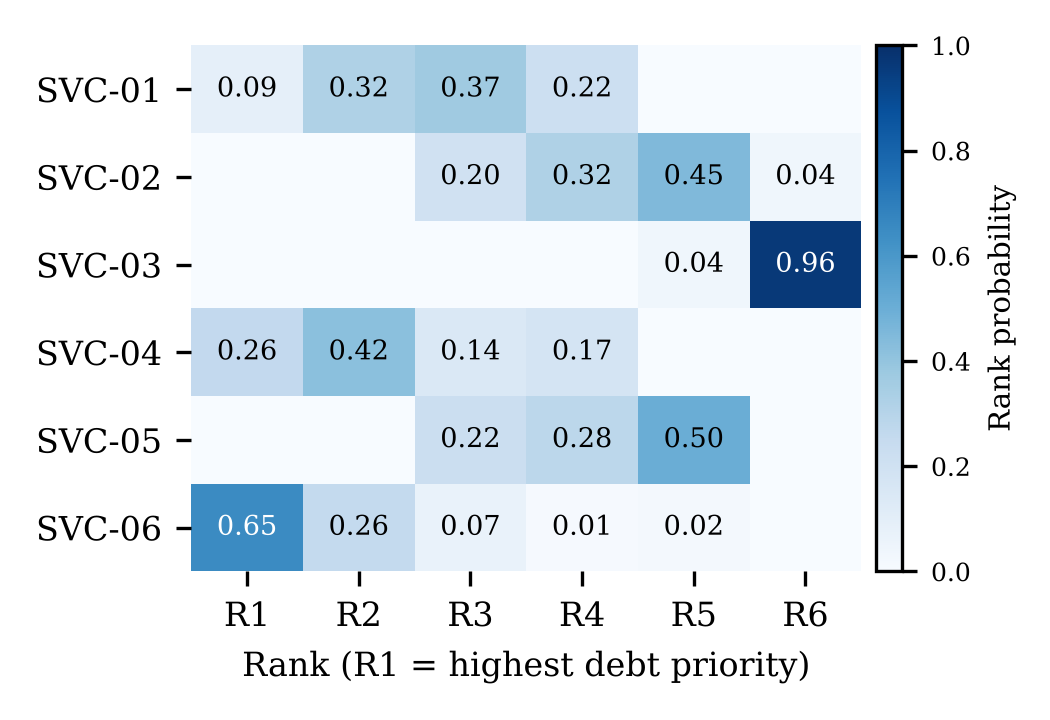
\includegraphics[width=1\linewidth,height=\textheight,keepaspectratio]{figures/fig_rank_acceptability.png}

}

\caption{\label{fig-rankacc}Rank-acceptability distribution for 2025
under absolute-mode TOPSIS across 20,000 weight vectors sampled
uniformly from the Dirichlet simplex (seed 50). Cells give the
probability that a service occupies a given rank.}

\end{figure}%

Repeating the analysis on 2024 data yields a flatter distribution.
SVC-03 occupies the lowest rank in 72.0\% of weightings rather than
96.4\%, and the top rank spreads across three services, with SVC-04
taking it in 42.6\% of draws, SVC-06 in 32.3\% and SVC-02 in 25.1\%.
This mirrors the weaker 2024 figures in Section~\ref{sec-stability} and
has the same cause, the more compressed 2024 profiles, confirming that
weight sensitivity here is a property of the data rather than of the
method.

\subsection{Indicator Independence}\label{sec-independence}

A composite only adds information over its parts if the parts are not
redundant. Table~\ref{tbl-correlation} reports Spearman rank
correlations among the five indicators across the twelve service-years
in the dataset. Three clusters emerge. Incident frequency and CFR are
strongly correlated (\(\rho = 0.84\)), which is the shared incident
numerator noted in Section~\ref{sec-indicators}. Patch recency and
unsupported component months are almost perfectly inversely related
(\(\rho = -0.98\)), since both describe the lifecycle state of the same
component stack. MTTR is uncorrelated with every other indicator
(absolute \(\rho \leq 0.36\)). The five indicators therefore carry three
distinct signals, namely incident load, recovery capability and
lifecycle exposure, rather than five. This matters for interpretation.
Under equal weights the incident and lifecycle clusters each receive
0.40 of the total weight and recovery 0.20, so the baseline is not as
neutral as it appears, and the differential configuration, which raises
MTTR to 0.30, partly corrects this. Two correlated indicators also
overweight that signal in the vector-normalised distance. The clusters
do not invalidate the design, because each indicator remains the only
observable for its particular debt dimension in
Table~\ref{tbl-indicators-lit}, but they explain why the ranking
resolves cleanly at the extremes and less so in the middle, and they
motivate a cluster-level weighting as future work. With twelve
observations only the two strong correlations reach conventional
significance (\(p < 0.001\)), and the rest should be read as
descriptive.

\begin{table}

\caption{\label{tbl-correlation}Spearman rank correlations among the
five indicators, twelve service-years (2024 and 2025 pooled)}

\centering{

\scriptsize
\setlength{\tabcolsep}{5pt}
\begin{tabular}{@{}lrrrrr@{}}
\toprule
 & Inc. freq. & MTTR & CFR & Patch rec. & Unsup. months \\
\midrule
Inc. freq. & 1 & & & & \\
MTTR & 0.13 & 1 & & & \\
CFR & 0.84 & $-$0.36 & 1 & & \\
Patch rec. & 0.20 & $-$0.08 & 0.21 & 1 & \\
Unsup. months & $-$0.20 & 0.02 & $-$0.17 & $-$0.98 & 1 \\
\bottomrule
\end{tabular}

}

\end{table}%

\subsection{Practical Validity}\label{sec-practical}

Three services illustrate what the rankings capture. SVC-06 holds rank 1
under both configurations and both TOPSIS modes, pairing the portfolio's
heaviest per-component lifecycle exposure with the worst CFR, the worst
patch recency and the second-highest incident count.
Table~\ref{tbl-indicators-lit} places this debt across the
infrastructure lifecycle, vulnerability, process and architectural
dimensions. SVC-06 is worst or near-worst on four of the five
indicators, which is why it is robustly top. SVC-01 holds rank 3 and is
the multi-criteria exemplar: a modest incident count masks the
portfolio's highest MTTR, its second-worst patch recency and its
second-worst per-component exposure, the signature of infrastructure and
vulnerability debt behind a quiet incident profile. SVC-04 holds rank 2
with the mirror-image profile of the highest incident frequency, a high
MTTR and a high CFR, yet no unsupported components and full patch
recency, the indicators of architectural and process debt
\citeproc{ref-detoledoReducingIncidentsMicroservices2021}{{[}23{]}},
\citeproc{ref-nordExamplesTechnicalDebts2021}{{[}30{]}}. SVC-03 has the
lowest priority in every run and is the reference case for a
well-maintained service.

A cross-sectional design cannot show whether these metrics are
downstream effects of TD severity or arise from other operational
factors. Proxy validity is therefore judged by how far each profile
converges with theory, not by a demonstrated causal mechanism. Each
profile matches a debt pattern the literature documents
\citeproc{ref-hakiDigitalNudgingTechnical2023}{{[}5{]}},
\citeproc{ref-ramasubbuControllingTechnicalDebt2021}{{[}6{]}},
\citeproc{ref-nordExamplesTechnicalDebts2021}{{[}30{]}}, and the
profiles are distinct from one another rather than versions of a single
underlying deficiency. The match is a consistency check rather than an
independent test, because the ranking is computed from the same
indicators that form each profile.

\section{Discussion}\label{sec-discussion}

\subsection{Answers to the Research
Questions}\label{answers-to-the-research-questions}

RQ1 asked how TD can be prioritised quantitatively at the service level
from operational data. The framework itself is the answer. Five
indicators, three from ITSM and two from the CMDB, feed a TOPSIS model
that orders services by debt priority without any recourse to source
code. Its multi-criteria form is not decorative. The ranking diverges
from an incident-only view, modestly in 2025 and sharply in 2024, a
divergence that would have collapsed had the indicators moved together.
SVC-01 rises on infrastructure and patch debt an incident count ignores,
while SVC-05 falls on a clean infrastructure profile.

RQ2 asked to what extent operational metrics serve as valid proxies for
TD severity. The answer is: to a demonstrable but bounded extent. Each
indicator's link to a debt dimension is inherited from the literature
rather than established here. What this study adds is evidence that the
composite behaves as an instrument should. The ranked profiles are
differentiated rather than one deficiency in disguise, no single
indicator reproduces the ordering, and the correlation analysis shows
that the indicator set carries three distinct signals rather than one.
This is a necessary condition for the proxy claim, not a sufficient one.
Criterion validity cannot be established, since no independent measure
of non-code debt exists to validate against. The proxy relationship
therefore remains a proposition that survived every test this design
allows.

RQ3 asked how stable the rankings are under weight perturbation. They
are stable at both extremes and concentrated but weight-dependent at the
top. The two configurations agree closely in 2025 (\(\tau = 0.867\)),
and across 20,000 Monte Carlo weightings SVC-03 is last in 96.4\% of
draws and SVC-06 first in 65.1\%, ceding rank 1 only to SVC-04 or
SVC-01. The 2024 profiles are more compressed and divide the
high-priority ranks more evenly, marking the line between what the
framework settles and what remains a managerial judgement.

\subsection{Implications for Research}\label{implications-for-research}

The contribution to knowledge is threefold. Empirically, the study
provides what we believe is the first application of TOPSIS to live ITSM
and CMDB records for TD prioritisation in financial trading IT,
addressing the absence of validated quantitative approaches identified
by Lenarduzzi et al.
\citeproc{ref-lenarduzziSystematicLiteratureReview2021}{{[}7{]}} and
contributing an operational dataset from a securities trading
environment, which is currently absent from the literature.
Conceptually, it contributes an operationally defined indicator set with
an explicit literature mapping to debt dimensions and evidence on how
the set behaves under evaluation. Methodologically, the evaluation
produced an unexpected finding. Vector-normalised TOPSIS can reward a
service simply for being the worst in the sample, whereas VIKOR's regret
term and the absolute-mode variant do not, and in the 2024 data this
difference reordered the top-priority services. The two formulations
encode different positions on whether debt dimensions are compensatory,
and the division of labour proposed in Section~\ref{sec-absolutemode}, a
relative primary signal certified by an absolute-frame companion, is a
design lesson that extends beyond this case.

\subsection{Implications for Practice}\label{implications-for-practice}

For the case organisation and similar institutions, the framework
converts data already held in routine ITSM and CMDB records into an
auditable priority ordering. Its primary use is portfolio oversight.
Services are currently assessed one at a time, by different teams and on
different evidence, so no consistent view of debt-related status exists
across the portfolio. The ranking supplies one, and the profiles behind
it show why each service sits where it does, letting portfolio managers
and senior management argue remediation budgets and vendor conversations
from a common picture. It also surfaces the debt current governance is
most likely to miss, such as a service that looks comparatively quiet on
incidents yet carries the highest MTTR and substantial lifecycle
exposure once that exposure is measured per component.

The regulatory relevance is narrower than compliance. FINMA Circular
2023/1 places ICT risk management under board-level oversight
\citeproc{ref-finmaCircular202312024}{{[}4{]}}, and unsupported
components and patch delay are ICT risks in that sense. The framework
was not designed against the circular, but it provides a consolidated
view of some of the exposures the institution must oversee in any case.
The framework is also transparent and reproducible by construction.
Indicator definitions, normalisation, weights and computation are stated
in full, so any reported ranking can be recomputed and independently
verified. Proprietary static analysis tools, by contrast, rest on
rulesets that users cannot inspect and that disagree on the same
codebase
\citeproc{ref-amanatidisEvaluatingAgreementTechnical2020}{{[}9{]}}. In a
regulated setting, a verifiable ranking is easier to defend before
auditors than an opaque score.

Two conditions govern its use. The scores are ordinal decision-support
signals, not measurements of debt. They also describe services, not
teams, since high-debt profiles typically reflect historical design
decisions rather than current custodians
\citeproc{ref-ahmadTechnicalDebtNot2026}{{[}15{]}}. Priority scores can
influence budgets, staffing and post-incident accountability in
regulated institutions, so any operational use beyond the agreed
portfolio management scope should require a separate governance
decision.

\subsection{Threats to Validity}\label{threats-to-validity}

Construct validity is the central limitation. Every strand of the
evaluation uses the same dataset and indicators that built the
framework, so the triangulation and baseline comparisons establish
convergent and discriminant validity but not criterion validity. The
indicators are proxies whose link to debt dimensions is inherited from
the literature, and Section~\ref{sec-independence} shows that they form
three correlated clusters rather than five independent measures, so the
equal-weight baseline implicitly weights incident load and lifecycle
exposure twice as heavily as recovery capability. Recording-practice
variation across teams can also compress scores where informal incident
handling is common.

Internal validity is constrained by the cross-sectional design. The
framework captures a snapshot, so a service in the middle of remediation
may look worse than warranted and recently remediated services may be
under-ranked. Conclusion validity is limited by the six-service
demonstration set. Weight stability is a quality criterion, yet its
strong 2024 agreement of \(\tau = 0.733\) still returns \(p = 0.056\),
slightly above the conventional threshold, which reflects the small
sample rather than weak agreement. The method disagreement over the
single top rank in 2024 adds a further boundary. It turns on whether
concentrated structural exposure is judged more urgent than diffuse
operational debt, a compensability judgement the framework informs
rather than settles.

External validity is bounded by the single-site design. Indicator
weights, absolute-mode bounds and the TOPSIS configuration are
calibrated for one organisation and should not be transferred without
revalidation. The five indicators also do not exhaust all dimensions of
operational TD, since documentation, test coverage and architectural
coupling were excluded on data availability grounds.

\section{Conclusion and Future Work}\label{sec-conclusion}

Vendor-dominated trading IT lacked a quantitative, service-level
instrument for prioritising technical debt, because code-centric tools
cannot operate where source code is inaccessible. This paper has
presented a framework that fills that gap. Five operational indicators
were derived from the literature, mapped to TD dimensions and
operationalised from two years of live ITSM and CMDB records at a
regulated Swiss financial institution. A TOPSIS model ranked six
production services under two weight configurations and two observation
years, and the ranking was tested from six directions. It proved stable
under weight variation, was reproduced by alternative methods, diverged
from a single-criterion baseline, survived service removal under an
absolute-mode variant, rested on three distinct indicator signals, and
was readable against differentiated service profiles. A Monte Carlo
exploration of 20,000 weightings showed that the lowest priority is
weight-invariant and the top priority concentrates on one service in two
thirds of weightings. The framework does not measure TD. It orders
services by the operational shadow debt casts, and within the limits
stated it does so reproducibly, defensibly and in a form a regulated
institution can act on.

Four directions follow. The first is external validation, replicating
the framework at further regulated institutions and comparing their
indicator weights and dimension mappings, to test the proxy proposition
beyond this case. The second is longitudinal evaluation with a lagged
design, tracking whether high-priority services later generate the
consequences the debt literature predicts
\citeproc{ref-bankerTechnicalDebtFirm2020}{{[}3{]}}, which is the route
to the criterion validity this design cannot reach. The third is
portfolio-wide deployment once indicator coverage is complete, replacing
the demonstration set with a live ranking and strengthening the
stability tests, since Kendall's \(\tau\) gains power with sample size.
The fourth is deriving the absolute-mode bounds from regulatory or
cross-industry end-of-support benchmarks rather than organisational
thresholds, making scores comparable between organisations as well as
between years. A fifth, prompted by the correlation structure in
Section~\ref{sec-independence}, is a cluster-level weighting that
assigns weight to incident load, recovery capability and lifecycle
exposure as signals before distributing it across their constituent
indicators.

\section*{Acknowledgment}\label{acknowledgment}
\addcontentsline{toc}{section}{Acknowledgment}

The authors thank the Head of Trading IT of the case organisation for
authorising access to the anonymised service management records and for
agreeing the governance scope of this study.

\section*{Data Availability}\label{data-availability}
\addcontentsline{toc}{section}{Data Availability}

The Python implementation of the standard and absolute-mode TOPSIS
procedures, the SAW and VIKOR comparators and the Monte Carlo analysis,
together with the anonymised decision matrices for both observation
years, are openly available at
\url{https://github.com/TobiZeier/MScProject/tree/main/code}. The
underlying ITSM and CMDB records cannot be shared because they are the
property of the case organisation.

\section*{Declaration of Competing
Interest}\label{declaration-of-competing-interest}
\addcontentsline{toc}{section}{Declaration of Competing Interest}

The second author is employed in the trading IT division of the case
organisation. The organisation had no role in the design of the study,
the analysis or the decision to publish, and no outputs were shared with
service teams during the research period. The first author declares no
competing interests.

\section*{References}\label{references}
\addcontentsline{toc}{section}{References}

\phantomsection\label{refs}
\begin{CSLReferences}{0}{0}
\bibitem[\citeproctext]{ref-cunninghamWyCashPortfolioManagement1992}
\CSLLeftMargin{{[}1{]} }%
\CSLRightInline{W. Cunningham,
{``\href{https://doi.org/10.1145/157710.157715}{The {WyCash} portfolio
management system},''} \emph{ACM SIGPLAN OOPS Messenger}, vol. 4, no. 2,
pp. 29--30, Oct. 1992. }

\bibitem[\citeproctext]{ref-kruchtenTechnicalDebtMetaphor2012}
\CSLLeftMargin{{[}2{]} }%
\CSLRightInline{P. Kruchten, R. L. Nord, and I. Ozkaya,
{``\href{https://doi.org/10.1109/MS.2012.167}{Technical {Debt}: {From
Metaphor} to {Theory} and {Practice}},''} \emph{IEEE Software}, vol. 29,
no. 6, pp. 18--21, Nov. 2012. }

\bibitem[\citeproctext]{ref-bankerTechnicalDebtFirm2020}
\CSLLeftMargin{{[}3{]} }%
\CSLRightInline{R. Banker, Y. Liang, and N. Ramasubbu,
{``\href{https://doi.org/10.1287/mnsc.2019.3542}{Technical {Debt} and
{Firm Performance}},''} \emph{Management Science}, vol. 67, no. 5, pp.
3174--3194, May 2021. }

\bibitem[\citeproctext]{ref-finmaCircular202312024}
\CSLLeftMargin{{[}4{]} }%
\CSLRightInline{FINMA, {``Operational risks and resilience: {Banks},''}
Swiss Financial Market Supervisory Authority FINMA, Bern, Switzerland,
Circular 2023/1, Dec. 2022 {[}Online{]}. Available:
\url{https://www.finma.ch/en/~/media/finma/dokumente/dokumentencenter/myfinma/rundschreiben/finma-rs-2023-01-20221207.pdf}.
{[}Accessed: 29-Mar-2026{]}}

\bibitem[\citeproctext]{ref-hakiDigitalNudgingTechnical2023}
\CSLLeftMargin{{[}5{]} }%
\CSLRightInline{K. Haki, A. Rieder, L. Buchmann, and A. W. Schneider,
{``\href{https://doi.org/10.1080/0960085X.2022.2088413}{Digital nudging
for technical debt management at {Credit Suisse}},''} \emph{European
Journal of Information Systems}, vol. 32, no. 1, pp. 64--80, Jan. 2023.
}

\bibitem[\citeproctext]{ref-ramasubbuControllingTechnicalDebt2021}
\CSLLeftMargin{{[}6{]} }%
\CSLRightInline{N. Ramasubbu and C. F. Kemerer,
{``\href{https://doi.org/10.1080/07421222.2021.1870377}{Controlling
{Technical Debt Remediation} in {Outsourced Enterprise Systems
Maintenance}: {An Empirical Analysis}},''} \emph{Journal of Management
Information Systems}, vol. 38, no. 1, pp. 4--28, Jan. 2021. }

\bibitem[\citeproctext]{ref-lenarduzziSystematicLiteratureReview2021}
\CSLLeftMargin{{[}7{]} }%
\CSLRightInline{V. Lenarduzzi, T. Besker, D. Taibi, A. Martini, and F.
Arcelli Fontana, {``\href{https://doi.org/10.1016/j.jss.2020.110827}{A
systematic literature review on {Technical Debt} prioritization:
{Strategies}, processes, factors, and tools},''} \emph{Journal of
Systems and Software}, vol. 171, p. 110827, Jan. 2021. }

\bibitem[\citeproctext]{ref-biazottoTechnicalDebtManagement2024}
\CSLLeftMargin{{[}8{]} }%
\CSLRightInline{J. P. Biazotto, D. Feitosa, P. Avgeriou, and E. Y.
Nakagawa,
{``\href{https://doi.org/10.1016/j.infsof.2023.107375}{Technical debt
management automation: {State} of the art and future perspectives},''}
\emph{Information and Software Technology}, vol. 167, p. 107375, Mar.
2024. }

\bibitem[\citeproctext]{ref-amanatidisEvaluatingAgreementTechnical2020}
\CSLLeftMargin{{[}9{]} }%
\CSLRightInline{T. Amanatidis, N. Mittas, A. Moschou, A. Chatzigeorgiou,
A. Ampatzoglou, and L. Angelis,
{``\href{https://doi.org/10.1007/s10664-020-09869-w}{Evaluating the
agreement among technical debt measurement tools: Building an empirical
benchmark of technical debt liabilities},''} \emph{Empirical Software
Engineering}, vol. 25, no. 5, pp. 4161--4204, Sep. 2020. }

\bibitem[\citeproctext]{ref-forsgrenAccelerate2018}
\CSLLeftMargin{{[}10{]} }%
\CSLRightInline{N. Forsgren, J. Humble, and G. Kim, \emph{Accelerate:
{The Science} of {Lean Software} and {DevOps}: {Building} and {Scaling
High Performing Technology Organizations}}. Portland, OR, USA: IT
Revolution Press, 2018. }

\bibitem[\citeproctext]{ref-hwangMultipleAttributeDecision1981}
\CSLLeftMargin{{[}11{]} }%
\CSLRightInline{C.-L. Hwang and K. Yoon,
\emph{\href{https://doi.org/10.1007/978-3-642-48318-9}{Multiple
{Attribute Decision Making}: {Methods} and {Applications}}}, vol. 186.
Berlin, Germany: Springer, 1981. }

\bibitem[\citeproctext]{ref-hevnerDesignScienceInformation2004}
\CSLLeftMargin{{[}12{]} }%
\CSLRightInline{A. R. Hevner, S. T. March, J. Park, and S. Ram,
{``\href{https://doi.org/10.2307/25148625}{Design {Science} in
{Information Systems Research}},''} \emph{MIS Quarterly}, vol. 28, no.
1, pp. 75--105, Mar. 2004. }

\bibitem[\citeproctext]{ref-mcconnellManagingTechnicalDebt2008}
\CSLLeftMargin{{[}13{]} }%
\CSLRightInline{S. McConnell, {``Managing {Technical Debt},''} Construx
Software, Bellevue, WA, USA, Best Practices White Paper, Jun. 2008
{[}Online{]}. Available:
\url{https://www.construx.com/wp-content/uploads/2019/02/CxWhitePaper_TechnicalDebt.pdf}.
{[}Accessed: 21-Mar-2026{]}}

\bibitem[\citeproctext]{ref-beskerTechnicalDebtEmpirical2020}
\CSLLeftMargin{{[}14{]} }%
\CSLRightInline{T. Besker, {``Technical {Debt}: {An} empirical
investigation of its harmfulness and on management strategies in
industry,''} PhD thesis, Chalmers University of Technology, Gothenburg,
Sweden, 2020 {[}Online{]}. Available:
\url{https://research.chalmers.se/publication/518318/file/518318_Fulltext.pdf}}

\bibitem[\citeproctext]{ref-ahmadTechnicalDebtNot2026}
\CSLLeftMargin{{[}15{]} }%
\CSLRightInline{M. O. Ahmad, V. Mandić, N. Taušan, A. Katin, and P.
Herath, {``\href{https://doi.org/10.1016/j.jss.2025.112719}{Technical
debt is not just technical: {An} industrial case study in large agile
software development},''} \emph{Journal of Systems and Software}, vol.
234, p. 112719, Apr. 2026. }

\bibitem[\citeproctext]{ref-vidoniInfiniteTechnicalDebt2022}
\CSLLeftMargin{{[}16{]} }%
\CSLRightInline{M. Vidoni, Z. Codabux, and F. H. Fard,
{``\href{https://doi.org/10.1016/j.jss.2022.111336}{Infinite technical
debt},''} \emph{Journal of Systems and Software}, vol. 190, p. 111336,
Aug. 2022. }

\bibitem[\citeproctext]{ref-kleinwaksTechnicalDebtSystems2023}
\CSLLeftMargin{{[}17{]} }%
\CSLRightInline{H. Kleinwaks, A. Batchelor, and T. H. Bradley,
{``\href{https://doi.org/10.1002/sys.21681}{Technical debt in systems
engineering: {A} systematic literature review},''} \emph{Systems
Engineering}, vol. 26, no. 5, pp. 675--687, Sep. 2023. }

\bibitem[\citeproctext]{ref-hanssenIdentifyingScalabilityDebt2019}
\CSLLeftMargin{{[}18{]} }%
\CSLRightInline{G. K. Hanssen, G. Brataas, and A. Martini,
{``\href{https://doi.org/10.1109/TechDebt.2019.00014}{Identifying
{Scalability Debt} in {Open Systems}},''} in \emph{2019 {IEEE}/{ACM
International Conference} on {Technical Debt} ({TechDebt})}, 2019, pp.
48--52. }

\bibitem[\citeproctext]{ref-yangTaxonomyTechnicalDebt2019}
\CSLLeftMargin{{[}19{]} }%
\CSLRightInline{Y. Yang, R. Michel, J. Wade, D. Verma, M. Törngren, and
T. Alelyani,
{``\href{https://doi.org/10.1016/j.procs.2019.05.061}{Towards a taxonomy
of technical debt for {COTS-intensive} cyber physical systems},''}
\emph{Procedia Computer Science}, vol. 153, pp. 108--117, 2019. }

\bibitem[\citeproctext]{ref-ampatzoglouSDK4EDPlatformTechnical2022}
\CSLLeftMargin{{[}20{]} }%
\CSLRightInline{A. Ampatzoglou, A. Chatzigeorgiou, E. M. Arvanitou, and
S. Bibi, {``\href{https://doi.org/10.1002/spe.3093}{{SDK4ED}: {A}
platform for technical debt management},''} \emph{Software: Practice and
Experience}, vol. 52, no. 8, pp. 1879--1902, 2022. }

\bibitem[\citeproctext]{ref-tornhillCodeRedBusiness2022}
\CSLLeftMargin{{[}21{]} }%
\CSLRightInline{A. Tornhill and M. Borg,
{``\href{https://doi.org/10.1145/3524843.3528091}{Code {Red}: {The
Business Impact} of {Code Quality}: {A Quantitative Study} of 39
{Proprietary Production Codebases}},''} in \emph{2022 {IEEE}/{ACM
International Conference} on {Technical Debt} ({TechDebt})}, 2022, pp.
11--20. }

\bibitem[\citeproctext]{ref-albuquerqueManagingTechnicalDebt2023}
\CSLLeftMargin{{[}22{]} }%
\CSLRightInline{D. Albuquerque \emph{et al.},
{``\href{https://doi.org/10.1109/TSE.2022.3214764}{Managing {Technical
Debt Using Intelligent Techniques}: {A Systematic Mapping Study}},''}
\emph{IEEE Transactions on Software Engineering}, vol. 49, no. 4, pp.
2202--2220, Apr. 2023. }

\bibitem[\citeproctext]{ref-detoledoReducingIncidentsMicroservices2021}
\CSLLeftMargin{{[}23{]} }%
\CSLRightInline{S. S. de Toledo, A. Martini, D. I. K. Sjøberg, A.
Przybyszewska, and J. S. Frandsen,
{``\href{https://doi.org/10.1109/SEAA53835.2021.00033}{Reducing
{Incidents} in {Microservices} by {Repaying Architectural Technical
Debt}},''} in \emph{2021 47th {Euromicro Conference} on {Software
Engineering} and {Advanced Applications} ({SEAA})}, 2021, pp. 196--205.
}

\bibitem[\citeproctext]{ref-alfayezHowSonarQubeidentifiedTechnical2023}
\CSLLeftMargin{{[}24{]} }%
\CSLRightInline{R. Alfayez, R. Winn, W. Alwehaibi, E. Venson, and B.
Boehm, {``\href{https://doi.org/10.1016/j.infsof.2023.107147}{How
{SonarQube-identified} technical debt is prioritized: {An} exploratory
case study},''} \emph{Information and Software Technology}, vol. 156, p.
107147, Apr. 2023. }

\bibitem[\citeproctext]{ref-pinaTechnicalDebtPrioritization2022}
\CSLLeftMargin{{[}25{]} }%
\CSLRightInline{D. Pina, C. Seaman, and A. Goldman,
{``\href{https://doi.org/10.1145/3524843.3528096}{Technical {Debt
Prioritization}: {A Developer}'s {Perspective}},''} in \emph{2022
{IEEE}/{ACM International Conference} on {Technical Debt} ({TechDebt})},
2022, pp. 46--55. }

\bibitem[\citeproctext]{ref-wieseITManagersPerspective2023}
\CSLLeftMargin{{[}26{]} }%
\CSLRightInline{M. Wiese and K. Borowa,
{``\href{https://doi.org/10.1016/j.jss.2023.111700}{{IT} managers'
perspective on {Technical Debt Management}},''} \emph{Journal of Systems
and Software}, vol. 202, p. 111700, Aug. 2023. }

\bibitem[\citeproctext]{ref-stochelBusinessdrivenTechnicalDebt2023}
\CSLLeftMargin{{[}27{]} }%
\CSLRightInline{M. G. Stochel, T. Borek, M. R. Wawrowski, and P. Chołda,
{``\href{https://doi.org/10.1016/j.infsof.2023.107333}{Business-driven
technical debt management using {Continuous Debt Valuation Approach}
({CoDVA})},''} \emph{Information and Software Technology}, vol. 164, p.
107333, Dec. 2023. }

\bibitem[\citeproctext]{ref-rollandExploringTensionsManagement2021}
\CSLLeftMargin{{[}28{]} }%
\CSLRightInline{K.-H. Rolland and K. Lyytinen,
{``\href{https://doi.org/10.24251/HICSS.2021.807}{Exploring the
{Tensions Between Management} of {Architectural Debt} and {Digital
Innovation}: {The Case} of a {Financial Organization}},''} in
\emph{Proceedings of the 54th {Hawaii International Conference} on
{System Sciences} ({HICSS})}, 2021, pp. 6722--6732. }

\bibitem[\citeproctext]{ref-rinta-kahilaGettingTrappedTechnical2023}
\CSLLeftMargin{{[}29{]} }%
\CSLRightInline{T. Rinta-Kahila, E. Penttinen, and K. Lyytinen,
{``\href{https://doi.org/10.25300/MISQ/2022/16711}{Getting {Trapped} in
{Technical Debt}: {Sociotechnical Analysis} of a {Legacy System}'s
{Replacement}},''} \emph{MIS Quarterly}, vol. 47, no. 1, pp. 1--32, Mar.
2023. }

\bibitem[\citeproctext]{ref-nordExamplesTechnicalDebts2021}
\CSLLeftMargin{{[}30{]} }%
\CSLRightInline{R. L. Nord, I. Ozkaya, and C. Woody, {``Examples of
{Technical Debt}'s {Cybersecurity Impact},''} Software Engineering
Institute, Carnegie Mellon University, Pittsburgh, PA, USA, Technical
Report, Jul. 2021 {[}Online{]}. Available:
\url{https://apps.dtic.mil/sti/trecms/pdf/AD1144728.pdf}. {[}Accessed:
27-Apr-2026{]}}

\bibitem[\citeproctext]{ref-paudelExploringRelationshipTechnical2025}
\CSLLeftMargin{{[}31{]} }%
\CSLRightInline{B. Paudel, J. Gonzalez-Huerta, E. Zabardast, and E.
Klotins,
{``\href{https://doi.org/10.1109/SANER64311.2025.00071}{Exploring the
{Relationship Between Technical Debt} and {Lead Time}: {An Industrial
Case Study}},''} in \emph{2025 {IEEE International Conference} on
{Software Analysis}, {Evolution} and {Reengineering} ({SANER})}, 2025,
pp. 693--703. }

\bibitem[\citeproctext]{ref-nielsenITPortfolioManagement2022}
\CSLLeftMargin{{[}32{]} }%
\CSLRightInline{M. E. Nielsen and S. Skaarup,
{``\href{https://doi.org/10.1145/3494193.3494296}{{IT Portfolio}
management as a framework for managing {Technical Debt}: {Theoretical}
framework applied on a case study},''} in \emph{Proceedings of the 14th
{International Conference} on {Theory} and {Practice} of {Electronic
Governance} ({ICEGOV} 2021)}, 2022, pp. 89--96. }

\bibitem[\citeproctext]{ref-tizioSoftwareUpdatesStrategies2023}
\CSLLeftMargin{{[}33{]} }%
\CSLRightInline{G. Di Tizio, M. Armellini, and F. Massacci,
{``\href{https://doi.org/10.1109/TSE.2022.3176674}{Software {Updates
Strategies}: {A Quantitative Evaluation Against Advanced Persistent
Threats}},''} \emph{IEEE Transactions on Software Engineering}, vol. 49,
no. 3, pp. 1359--1373, Mar. 2023. }

\bibitem[\citeproctext]{ref-markkanenPatchManagementPlanning2023}
\CSLLeftMargin{{[}34{]} }%
\CSLRightInline{V. Markkanen and T. Frantti,
{``\href{https://doi.org/10.1109/DSA59317.2023.00018}{Patch management
planning: {Towards} one-to-one policy},''} in \emph{2023 10th
{International Conference} on {Dependable Systems} and {Their
Applications} ({DSA})}, 2023, pp. 60--69. }

\bibitem[\citeproctext]{ref-nursePatchNotPatch2025}
\CSLLeftMargin{{[}35{]} }%
\CSLRightInline{J. R. C. Nurse,
{``\href{https://doi.org/10.1007/978-3-031-92833-8_16}{To {Patch} or
{Not} to {Patch}: {Motivations}, {Challenges}, and {Implications} for
{Cybersecurity}},''} in \emph{{HCI} for {Cybersecurity}, {Privacy} and
{Trust} ({HCI-CPT} 2025)}, 2025, pp. 265--281. }

\bibitem[\citeproctext]{ref-kulaReleasingFastSlow2019}
\CSLLeftMargin{{[}36{]} }%
\CSLRightInline{E. Kula, A. Rastogi, H. Huijgens, A. van Deursen, and G.
Gousios, {``\href{https://doi.org/10.1145/3338906.3338978}{Releasing
fast and slow: {An} exploratory case study at {ING}},''} in
\emph{Proceedings of the 27th {ACM Joint Meeting} on {European Software
Engineering Conference} and {Symposium} on the {Foundations} of
{Software Engineering} ({ESEC}/{FSE} 2019)}, 2019, pp. 785--795. }

\bibitem[\citeproctext]{ref-ramasubbuManagingTechnicalDebt2015}
\CSLLeftMargin{{[}37{]} }%
\CSLRightInline{N. Ramasubbu, C. F. Kemerer, and C. J. Woodard,
{``\href{https://doi.org/10.1109/MS.2015.45}{Managing {Technical Debt}:
{Insights} from {Recent Empirical Evidence}},''} \emph{IEEE Software},
vol. 32, no. 2, pp. 22--25, Mar. 2015. }

\bibitem[\citeproctext]{ref-ciardielloComparisonTOPSISSAW2023}
\CSLLeftMargin{{[}38{]} }%
\CSLRightInline{F. Ciardiello and A. Genovese,
{``\href{https://doi.org/10.1007/s10479-023-05339-w}{A comparison
between {TOPSIS} and {SAW} methods},''} \emph{Annals of Operations
Research}, vol. 325, no. 2, pp. 967--994, Jun. 2023. }

\bibitem[\citeproctext]{ref-zanakisMultiattributeDecisionMaking1998}
\CSLLeftMargin{{[}39{]} }%
\CSLRightInline{S. H. Zanakis, A. Solomon, N. Wishart, and S. Dublish,
{``\href{https://doi.org/10.1016/S0377-2217(97)00147-1}{Multi-attribute
decision making: {A} simulation comparison of select methods},''}
\emph{European Journal of Operational Research}, vol. 107, no. 3, pp.
507--529, Jun. 1998. }

\bibitem[\citeproctext]{ref-garcia-cascalesRankReversalTOPSIS2012}
\CSLLeftMargin{{[}40{]} }%
\CSLRightInline{M. S. García-Cascales and M. T. Lamata,
{``\href{https://doi.org/10.1016/j.mcm.2011.12.022}{On rank reversal and
{TOPSIS} method},''} \emph{Mathematical and Computer Modelling}, vol.
56, no. 5--6, pp. 123--132, Sep. 2012. }

\bibitem[\citeproctext]{ref-yangIngeniousSolutionRank2020}
\CSLLeftMargin{{[}41{]} }%
\CSLRightInline{W. Yang,
{``\href{https://doi.org/10.1155/2020/9676518}{Ingenious {Solution} for
the {Rank Reversal Problem} of {TOPSIS Method}},''} \emph{Mathematical
Problems in Engineering}, vol. 2020, p. 9676518, 2020. }

\bibitem[\citeproctext]{ref-shekhovtsovComparativeCaseStudy2020}
\CSLLeftMargin{{[}42{]} }%
\CSLRightInline{A. Shekhovtsov and W. Sałabun,
{``\href{https://doi.org/10.1016/j.procs.2020.09.014}{A comparative case
study of the {VIKOR} and {TOPSIS} rankings similarity},''}
\emph{Procedia Computer Science}, vol. 176, pp. 3730--3740, 2020. }

\bibitem[\citeproctext]{ref-grecoMethodologicalFrameworkComposite2019}
\CSLLeftMargin{{[}43{]} }%
\CSLRightInline{S. Greco, A. Ishizaka, M. Tasiou, and G. Torrisi,
{``\href{https://doi.org/10.1007/s11205-017-1832-9}{On the
{Methodological Framework} of {Composite Indices}: {A Review} of the
{Issues} of {Weighting}, {Aggregation}, and {Robustness}},''}
\emph{Social Indicators Research}, vol. 141, no. 1, pp. 61--94, Jan.
2019. }

\bibitem[\citeproctext]{ref-albarakManagingTechnicalDebt2022}
\CSLLeftMargin{{[}44{]} }%
\CSLRightInline{M. Albarak, R. Bahsoon, I. Ozkaya, and R. L. Nord,
{``\href{https://doi.org/10.1109/TSE.2020.3001339}{Managing {Technical
Debt} in {Database Normalization}},''} \emph{IEEE Transactions on
Software Engineering}, vol. 48, no. 3, pp. 755--772, Mar. 2022. }

\bibitem[\citeproctext]{ref-zytoonDecisionSupportModel2020}
\CSLLeftMargin{{[}45{]} }%
\CSLRightInline{M. A. Zytoon,
{``\href{https://doi.org/10.1109/ACCESS.2020.2991179}{A {Decision
Support Model} for {Prioritization} of {Regulated Safety Inspections
Using Integrated Delphi}, {AHP} and {Double-Hierarchical TOPSIS
Approach}},''} \emph{IEEE Access}, vol. 8, pp. 83444--83464, 2020. }

\bibitem[\citeproctext]{ref-khanIntegratedMethodologyRanking2022}
\CSLLeftMargin{{[}46{]} }%
\CSLRightInline{S. Khan and L. Purohit,
{``\href{https://doi.org/10.1109/CSNT54456.2022.9787620}{An {Integrated
Methodology} of {Ranking Based} on {PROMETHEE-CRITIC} and
{TOPSIS-CRITIC} in {Web Service Domain}},''} in \emph{2022 {IEEE} 11th
{International Conference} on {Communication Systems} and {Network
Technologies} ({CSNT})}, 2022, pp. 335--340. }

\bibitem[\citeproctext]{ref-kellyThreePrinciplesPragmatism2020}
\CSLLeftMargin{{[}47{]} }%
\CSLRightInline{L. M. Kelly and M. Cordeiro,
{``\href{https://doi.org/10.1177/2059799120937242}{Three principles of
pragmatism for research on organizational processes},''}
\emph{Methodological Innovations}, vol. 13, no. 2, pp. 1--10, May 2020.
}

\bibitem[\citeproctext]{ref-peffersDesignScienceResearch2007}
\CSLLeftMargin{{[}48{]} }%
\CSLRightInline{K. Peffers, T. Tuunanen, M. A. Rothenberger, and S.
Chatterjee, {``\href{https://doi.org/10.2753/MIS0742-1222240302}{A
{Design Science Research Methodology} for {Information Systems
Research}},''} \emph{Journal of Management Information Systems}, vol.
24, no. 3, pp. 45--77, Dec. 2007. }

\bibitem[\citeproctext]{ref-FederalActData2023}
\CSLLeftMargin{{[}49{]} }%
\CSLRightInline{Swiss Federal Assembly, \emph{Federal {Act} on {Data
Protection} ({FADP}), {SR} 235.1}. 2023 {[}Online{]}. Available:
\url{https://www.fedlex.admin.ch/eli/cc/2022/491/en}. {[}Accessed:
15-Apr-2026{]}}

\bibitem[\citeproctext]{ref-CodeConductBCS2022}
\CSLLeftMargin{{[}50{]} }%
\CSLRightInline{BCS, The Chartered Institute for IT, {``Code of
{Conduct} for {BCS Members},''} BCS, The Chartered Institute for IT,
Swindon, UK, Jun. 2022 {[}Online{]}. Available:
\url{https://www.bcs.org/media/2211/bcs-code-of-conduct.pdf}.
{[}Accessed: 15-Apr-2026{]}}

\bibitem[\citeproctext]{ref-ampatzoglouReusabilityIndexMeasure2018}
\CSLLeftMargin{{[}51{]} }%
\CSLRightInline{A. Ampatzoglou, S. Bibi, A. Chatzigeorgiou, P. Avgeriou,
and I. Stamelos,
{``\href{https://doi.org/10.1007/978-3-319-90421-4_3}{Reusability
{Index}: {A Measure} for {Assessing Software Assets Reusability}},''} in
\emph{New {Opportunities} for {Software Reuse}}, vol. 10826, R. Capilla,
B. Gallina, and C. Cetina, Eds. Cham, Switzerland: Springer, 2018, pp.
43--58. }

\bibitem[\citeproctext]{ref-nardoToolsCompositeIndicators2005}
\CSLLeftMargin{{[}52{]} }%
\CSLRightInline{M. Nardo, M. Saisana, A. Saltelli, and S. Tarantola,
{``Tools for {Composite Indicators Building},''} European Commission,
Joint Research Centre, Ispra, Italy, Technical Report EUR 21682 EN, 2005
{[}Online{]}. Available:
\url{https://publications.jrc.ec.europa.eu/repository/handle/JRC31473}.
{[}Accessed: 31-Jul-2026{]}}

\bibitem[\citeproctext]{ref-pandeyReviewTOPSISMethod2023}
\CSLLeftMargin{{[}53{]} }%
\CSLRightInline{V. Pandey, Komal, and H. Dincer,
{``\href{https://doi.org/10.1007/s00500-023-09011-0}{A review on
{TOPSIS} method and its extensions for different applications with
recent development},''} \emph{Soft Computing}, vol. 27, no. 23, pp.
18011--18039, Dec. 2023. }

\bibitem[\citeproctext]{ref-shekhovtsovHowStronglyRank2021}
\CSLLeftMargin{{[}54{]} }%
\CSLRightInline{A. Shekhovtsov,
{``\href{https://doi.org/10.1016/j.procs.2021.09.235}{How strongly do
rank similarity coefficients differ used in decision making
problems?}''} \emph{Procedia Computer Science}, vol. 192, pp.
4570--4577, 2021. }

\bibitem[\citeproctext]{ref-chenRolesChallengesMerits2023}
\CSLLeftMargin{{[}55{]} }%
\CSLRightInline{O. Y. Chén \emph{et al.},
{``\href{https://doi.org/10.1016/j.patter.2023.100878}{The roles,
challenges, and merits of the p value},''} \emph{Patterns}, vol. 4, no.
12, p. 100878, Dec. 2023. }

\bibitem[\citeproctext]{ref-thienOvercomingLimitationsRAPS2024}
\CSLLeftMargin{{[}56{]} }%
\CSLRightInline{N. V. Thien, H. T. Dung, and D. D. Trung,
{``\href{https://doi.org/10.48084/etasr.7909}{Overcoming the
{Limitations} of the {RAPS Method} by identifying {Alternative Data
Normalization Methods}},''} \emph{Engineering, Technology \& Applied
Science Research}, vol. 14, no. 4, pp. 15745--15750, Aug. 2024. }

\end{CSLReferences}


% Can use something like this to put references on a page
% by themselves when using endfloat and the captionsoff option.
\ifCLASSOPTIONcaptionsoff
  \newpage
\fi

% trigger a \newpage just before the given reference
% number - used to balance the columns on the last page
% adjust value as needed - may need to be readjusted if
% the document is modified later
%\IEEEtriggeratref{8}
% The "triggered" command can be changed if desired:
%\IEEEtriggercmd{\enlargethispage{-5in}}

% Uncomment when use biblatex with style=ieee
%\renewcommand{\bibfont}{\footnotesize} % for IEEE bibfont size

\pagebreak[3]
% that's all folks
\end{document}

